% Converted from reference/DB4OFlare (MadCap Flare, Java target)

\chapter{Basics Operations \& Concepts}
\label{ref:basics}

This topic gives you an overview of the most important and basic features of db4o. First add db4o to your project. db4o doesn't need a complex setup. It's just a library which you can add to your project. \hyperref[ref:basics-getting-started]{See "Getting Started"} (p.~\pageref{ref:basics-getting-started})

\section*{Basic Operations}

The basic operations are unsurprisingly, storing, updating, querying and deleting objects. \hyperref[ref:basics-object-container]{See "The Basic Operations"} (p.~\pageref{ref:basics-object-container})

\begin{lstlisting}
ObjectContainer container = Db4oEmbedded.openFile("databaseFile.db4o");
try {
    // store a new pilot
    Pilot pilot = new Pilot("Joe");
    container.store(pilot);

    // query for pilots
    List<Pilot> pilots = container.query(new Predicate<Pilot>() {
        @Override
        public boolean match(Pilot pilot) {
            return pilot.getName().startsWith("Jo");
        }
    });

    // update pilot
    Pilot toUpdate = pilots.get(0);
    toUpdate.setName("New Name");
    container.store(toUpdate);

    // delete pilot
    container.delete(toUpdate);
} finally {
    container.close();
}
\end{lstlisting}

{\small\itshape Db4oBasics.java: The basic operations\par}
\medskip

For more information about queries: \hyperref[ref:basics-querying]{See "Querying"} (p.~\pageref{ref:basics-querying})

\section*{Basic Concepts}

There are some basic concepts which are used in db4o. Understanding them helps you to understand how db4o behaves. Some behaviors are common behaviors which you expect from a database, like transactions and ACID properties. \hyperref[ref:basics-acid-and-transactions]{See "ACID Properties And Transactions"} (p.~\pageref{ref:basics-acid-and-transactions})

db4o manages objects by identity. This means db4o doesn't need additional id-field on your object. \hyperref[ref:basics-identity-concept]{See "Identity Concept"} (p.~\pageref{ref:basics-identity-concept})

Other concepts are more unique to db4o, like the activation concept, which controls which objects are loaded from the storage to memory. \hyperref[ref:basics-activation]{See "Activation Concept"} (p.~\pageref{ref:basics-activation}). The same principals are also applied when updating (\hyperref[ref:basics-update-concept]{See "Update Concept"} (p.~\pageref{ref:basics-update-concept})  ) or deletion objects (\hyperref[ref:basics-delete-behavior]{See "Delete Behavior")} (p.~\pageref{ref:basics-delete-behavior})

\section{Getting Started}
\label{ref:basics-getting-started}

You can start using db4o within a few minutes following these few steps.

\subsection*{1. Get db4o}

db4o is maintained at \href{https://github.com/blakemcbride/db4o}{\nolinkurl{github.com/blakemcbride/db4o}}. Clone or download the repository; it contains the source code, the build and this manual.

\subsection*{2. Build db4o}

Build the jars as described in \href{https://github.com/blakemcbride/db4o/blob/master/BUILD.md}{\nolinkurl{BUILD.md}}. You need JDK 17 or newer and nothing else:

\begin{lstlisting}
./bld jar          # Linux, macOS
bld.cmd jar        # Windows
\end{lstlisting}

The jars are written to the target directory. \texttt{./bld javadoc} builds the API documentation into target/javadoc.

\subsection*{3. Adding db4o To Your Project}

The core of db4o is the single db4o-8.1-core.jar and has no additional dependencies. The other jars provide additional functionality \hyperref[ref:dependency-overview]{See "Dependency Overview".} (p.~\pageref{ref:dependency-overview}). You can also use db4o-8.1-all.jar, which includes every db4o feature.

To use db4o in your project you only need to add the required jars to your project and then you're ready to go.

Here is how to do this with Eclipse:

\begin{itemize}
\item Copy the db4o-*.jar to your projects library folder. If you don't have a library-folder yet, create one under your project. For example a folder called 'lib'.
\item Right-click on your project in the Package Explorer and choose "Refresh".
\item Right-click on your project in the Package Explorer again and choose "Properties".
\item Select "Java Build Path" in the tree view on the left.
\item Select the "Libraries" tabpage.
\item Click "Add JARs".
\item Your library folder should appear below your project. Choose the db4o-*.jars in this folder.
\item Confirm the changes.
\item Expand "Referenced Libraries" branch of your project in Package Explorer.
\item Select db4o-* library, right-click and open "Properties".
\item Select Javadoc Location in the list and browse to the target/javadoc folder of your db4o build.
\end{itemize}

\subsection*{4. Ready To Go}

That's it, now you're ready to go and can use db4o in your project.

\section{The Basic Operations}
\label{ref:basics-object-container}

The object container is the door to the database access. It's the starting point for all database operations.

\subsection{Access The Database}
\label{ref:basics-object-container:accessingdb}

The object container is the interface for accessing the database. To open the database you pass the file-name to the object container factory. Normally you should open an object container when the application starts and close it when it is shuts down.

\begin{lstlisting}
ObjectContainer container = Db4oEmbedded.openFile("databaseFile.db4o");
try {
    // use the object container
} finally {
    container.close();
}
\end{lstlisting}

{\small\itshape Db4oBasics.java: Open the object container to use the database\par}
\medskip

\subsection{Store Objects}
\label{ref:basics-object-container:storingobject}

Storing a object with db4o is extremely easy. Open the object container and pass your object to the store method and db4o will do the rest. There's no mapping required. db4o will read the class meta data, the read the object values with reflection and store the data.

\begin{lstlisting}
ObjectContainer container = Db4oEmbedded.openFile("databaseFile.db4o");
try {
    Pilot pilot = new Pilot("Joe");
    container.store(pilot);
} finally {
    container.close();
}
\end{lstlisting}

{\small\itshape Db4oBasics.java: Store an object\par}
\medskip

\subsection{Query The Database}
\label{ref:basics-object-container:queries}

Querying for objects is also easy. There are different query interfaces available with different benefits. \hyperref[ref:basics-querying]{See "Querying"} (p.~\pageref{ref:basics-querying})

The most natural query method is using \hyperref[ref:basics-querying-native-queries]{native queries} (p.~\pageref{ref:basics-querying-native-queries}). Basically you just pass in a instance of a predicate, which filters the objects out you want.

\begin{lstlisting}
ObjectContainer container = Db4oEmbedded.openFile("databaseFile.db4o");
try {
    List<Pilot> pilots = container.query(new Predicate<Pilot>() {
        public boolean match(Pilot o) {
            return o.getName().equals("Joe");
        }
    });
    for (Pilot pilot : pilots) {
        System.out.println(pilot.getName());
    }
} finally {
    container.close();
}
\end{lstlisting}

{\small\itshape Db4oBasics.java: Query for objects\par}
\medskip

\subsection{Update Objects}
\label{ref:basics-object-container:updateobjects}

Updating objects is also easy. First you query for the object which you want to update. Then you change the object and store it again in the database.

\begin{lstlisting}
ObjectContainer container = Db4oEmbedded.openFile("databaseFile.db4o");
try {
    List<Pilot> pilots = container.query(new Predicate<Pilot>() {
        public boolean match(Pilot o) {
            return o.getName().equals("Joe");
        }
    });
    Pilot aPilot = pilots.get(0);
    aPilot.setName("New Name");
    // update the pilot
    container.store(aPilot);
} finally {
    container.close();
}
\end{lstlisting}

{\small\itshape Db4oBasics.java: Update a pilot\par}
\medskip

\subsection{Delete Objects}
\label{ref:basics-object-container:deleteobjects}

Use the delete-operation to delete objects.

\begin{lstlisting}
ObjectContainer container = Db4oEmbedded.openFile("databaseFile.db4o");
try {
    List<Pilot> pilots = container.query(new Predicate<Pilot>() {
        public boolean match(Pilot o) {
            return o.getName().equals("Joe");
        }
    });
    Pilot aPilot = pilots.get(0);
    container.delete(aPilot);
} finally {
    container.close();
}
\end{lstlisting}

{\small\itshape Db4oBasics.java: Delete a object\par}
\medskip

\section{Querying}
\label{ref:basics-querying}

db4o supports different query mechanisms.

\hyperref[ref:basics-querying-native-queries]{Native Queries} (p.~\pageref{ref:basics-querying-native-queries}) is the main db4o query interface, recommended for general use.

\hyperref[ref:basics-querying-query-by-example]{Queries-By-Example} (p.~\pageref{ref:basics-querying-query-by-example}) are appropriate as a quick start for users who are still acclimating to storing and retrieving objects with db4o, but they are quite restrictive in functionality.

The \hyperref[ref:basics-querying-soda-query]{SODA Query} (p.~\pageref{ref:basics-querying-soda-query}) is the underlying internal API. It is provided for backward compatibility and it can be useful for dynamic generation of queries, where Native Queries are too strongly typed. There may be queries that will execute faster in SODA style, so it can be used to tune applications. You can also run snippets of custom query code as part of the SODA query,

Of course, you can mix these strategies as needed.

\subsection{Native Queries}
\label{ref:basics-querying-native-queries}

Wouldn't it be nice to write queries in the programming language that you are using? Wouldn't it be nice if all your query code was 100\% typesafe, 100\% compile-time checked and 100\% refactorable? Wouldn't it be nice if the full power of object-orientation could be used by calling methods from within queries?

Native queries allow you do to this. They bring you a nice query interface which doesn't rely on string literals. Because native queries simply use the semantics of your programming language, they are perfectly standardized and a safe choice for the future.

Native Queries are available for all platforms supported by db4o.

\subsubsection*{Principle}

Native Queries provide the ability to run one or more lines of code against all instances of a class. Native query expressions should return true to mark specific instances as part of the result set. db4o will attempt to \hyperref[ref:basics-querying-native-queries-native-query-optimization]{optimize native query} (p.~\pageref{ref:basics-querying-native-queries-native-query-optimization}) expressions where possible and use \hyperref[ref:basics-querying-soda-query]{internal query processor} (p.~\pageref{ref:basics-querying-soda-query}) to run them against indexes and without instantiating actual objects.

\subsubsection*{Dependencies}

For a good native query performance you need to add these jars to your project:db4o-8.1-nqopt.jar, db4o-8.1-instrumentation.jar, db4o-8.1-bloat.jar. \hyperref[ref:dependency-overview]{See "Dependency Overview"} (p.~\pageref{ref:dependency-overview})

\subsubsection*{Simple Example}

Let's look at how a simple native query will look like. See also a collection of example queries.

\begin{lstlisting}
ObjectSet<Pilot> result = container.query(new Predicate<Pilot>() {
    @Override
    public boolean match(Pilot pilot) {
        return pilot.getName().equals("John");
    }
});
\end{lstlisting}

{\small\itshape NativeQueryExamples.java: Check for equality of the name\par}
\medskip

\subsubsection*{Native Query Performance}

There's one drawback of native queries: Under the hood db4o tries to analyze native queries to convert them to \hyperref[ref:basics-querying-soda-query]{SODA} (p.~\pageref{ref:basics-querying-soda-query}). This is not possible for all queries. For some queries it is very difficult to analyze the flowgraph. In this case db4o will have to instantiate some of the persistent objects to actually run the native query code. db4o will try to analyze parts of native query expressions to keep object instantiation to the minimum.

The current state of the query optimization process is detailed in the chapter on \hyperref[ref:basics-querying-native-queries-native-query-optimization]{Native Query Optimization} (p.~\pageref{ref:basics-querying-native-queries-native-query-optimization})

\subsubsection*{Lazy Loaded Result Set}

db4o always returns lazy loaded result sets. That means the object container needs to stay open as long as you are using the result set. If you want use the result of a query after the object container has been closed, you need to copy the query result into a new collection first.

\subsubsection{Native Query Examples}
\label{ref:basics-querying-native-queries-native-query-examples}

Here's a collection of native query examples. These queries assume that there's a Pilot class with a name and age and a Car class with a pilot and name.

\paragraph{Equality}
\label{ref:basics-querying-native-queries-native-query-examples:equality}

This query shows you how compare a getter/setter for equality. In this example we compare the name of a person.

\begin{lstlisting}
ObjectSet<Pilot> result = container.query(new Predicate<Pilot>() {
    @Override
    public boolean match(Pilot pilot) {
        return pilot.getName().equals("John");
    }
});
\end{lstlisting}

{\small\itshape NativeQueryExamples.java: Check for equality of the name\par}
\medskip

\paragraph{Comparison}
\label{ref:basics-querying-native-queries-native-query-examples:comparison}

You can compare values with the usual comparison operators.

\begin{lstlisting}
ObjectSet<Pilot> result = container.query(new Predicate<Pilot>() {
    @Override
    public boolean match(Pilot pilot) {
        return pilot.getAge() > 18;
    }
});
\end{lstlisting}

{\small\itshape NativeQueryExamples.java: Compare values to each other\par}
\medskip

\paragraph{Query For Value Range}
\label{ref:basics-querying-native-queries-native-query-examples:valuerange}

Of course you can combine different comparisons. For example you can combine the greater and smaller than operators to check for a range of values.

\begin{lstlisting}
ObjectSet<Pilot> result = container.query(new Predicate<Pilot>() {
    @Override
    public boolean match(Pilot pilot) {
        return pilot.getAge() > 18 && pilot.getAge()<30;
    }
});
\end{lstlisting}

{\small\itshape NativeQueryExamples.java: Query for a particular rage of values\par}
\medskip

\paragraph{Combine Check With Logical Operators}
\label{ref:basics-querying-native-queries-native-query-examples:logicaloperators}

Of course you can combine a arbitrary set of conditions with logical operators.

\begin{lstlisting}
ObjectSet<Pilot> result = container.query(new Predicate<Pilot>() {
    @Override
    public boolean match(Pilot pilot) {
        return (pilot.getAge() > 18 && pilot.getAge()<30)
                || pilot.getName().equals("John");
    }
});
\end{lstlisting}

{\small\itshape NativeQueryExamples.java: Combine different comparisons with the logical operators\par}
\medskip

\paragraph{Query In Separate Class}
\label{ref:basics-querying-native-queries-native-query-examples:seperatequeryunit}

You can implement your query in a separate class  and then just us it where you need it. This is especially useful when you reuse the same query multiple times. Or you want to give your query a clear name for documentation purposes.

First write your  class :

\begin{lstlisting}
class AllJohns extends Predicate<Pilot> {
    @Override
    public boolean match(Pilot pilot) {
        return pilot.getName().equals("John");
    }
}
\end{lstlisting}

{\small\itshape AllJohns.java: Query as class\par}
\medskip

And then use it:

\begin{lstlisting}
ObjectSet<Pilot> result = container.query(new AllJohns());
\end{lstlisting}

{\small\itshape NativeQueryExamples.java: Use the predefined query\par}
\medskip

\paragraph{Arbitrary Code}
\label{ref:basics-querying-native-queries-native-query-examples:arbitrarycode}

In principal your query can contain any code and can do the most complex comparisons. However in practice the are limitations. The simple queries are \hyperref[ref:basics-querying-native-queries-native-query-optimization]{optimized and translated to SODA-queries} (p.~\pageref{ref:basics-querying-native-queries-native-query-optimization}). This is not possible for complex queries. If the query cannot be optimized, db4o will instantiate all objects and pass it to your query-object. This is a order of magnitude slower than a optimized native query and only feasible for smaller data sets.

\begin{lstlisting}
final List<Integer> allowedAges = Arrays.asList(18,20,33,55);
ObjectSet<Pilot> result = container.query(new Predicate<Pilot>() {
    @Override
    public boolean match(Pilot pilot) {
        return allowedAges.contains(pilot.getAge()) ||
               pilot.getName().toLowerCase().equals("John"); 
    }
});
\end{lstlisting}

{\small\itshape NativeQueryExamples.java: Arbitrary code\par}
\medskip

\subsubsection{Native Query Sorting}
\label{ref:basics-querying-native-queries-native-query-sorting}

Native Query syntax allows you to specify a comparator, which will be used to sort the results:

\begin{lstlisting}
final ObjectSet<Pilot> pilots = container.query(new Predicate<Pilot>() {
    @Override
    public boolean match(Pilot o) {
        return o.getAge() > 18;
    }
}, new QueryComparator<Pilot>() {
    public int compare(Pilot pilot, Pilot pilot1) {
        return pilot.getName().compareTo(pilot1.getName());
    }
});
\end{lstlisting}

{\small\itshape NativeQueriesSorting.java: Native query with sorting\par}
\medskip

\subsubsection{NQ Performance Characteristics}
\label{ref:basics-querying-native-queries-nq-performance-characteristics}

This overview shows which query operations perform well or badly on large datasets. It should give you an idea which operations can be used on large datasets and which operations can only be applied to small datasets.

Native queries are translated to SODA and therefore they share the same basic \hyperref[ref:basics-querying-soda-soda-performance-characteristics]{performance characteristics} (p.~\pageref{ref:basics-querying-soda-soda-performance-characteristics}).

\paragraph{Good Performance Characteristics}
\label{ref:basics-querying-native-queries-nq-performance-characteristics:goodperf}

For a good query performance fields which are used in a query have to be \hyperref[ref:basics-indexing]{indexed} (p.~\pageref{ref:basics-indexing}). Otherwise db4o needs to scan through all objects. With an index these operations should scale logarithmically with the amount of data. The following queries all assume that the fields are indexed.

\subparagraph*{Equals Operation on Indexed Field}

Simple equals operations on indexed fields' perform very well.

\begin{lstlisting}
final String criteria = Item.dataString(rnd.nextInt(NUMBER_OF_ITEMS));
final List<Item> result = container.query(new Predicate<Item>() {
    @Override
    public boolean match(Item o) {
        return o.getIndexedString().equals(criteria);
    }
});
\end{lstlisting}

{\small\itshape GoodPerformance.java: Equals operation\par}
\medskip

Not equals operations also do perform well. However a 'not equals' operation tends to return a large result which will slow down the query.

\begin{lstlisting}
final String criteria = Item.dataString(rnd.nextInt(NUMBER_OF_ITEMS));
final List<Item> result = container.query(new Predicate<Item>() {
    @Override
    public boolean match(Item o) {
        return !o.getIndexedString().equals(criteria);
    }
});
\end{lstlisting}

{\small\itshape GoodPerformance.java: Not equals operation\par}
\medskip

\subparagraph*{Navigation Queries on Index Field}

Queries which navigate along references are executed also efficiently, as long every field and reference is indexed.

However there's a catch to this: The reference field type has to be a concrete type. If a field type is a generic type, an interface or an object-type, then the query runs slow.

\begin{lstlisting}
final String criteria = Item.dataString(rnd.nextInt(NUMBER_OF_ITEMS));
final List<ItemHolder> result = container.query(new Predicate<ItemHolder>() {
    @Override
    public boolean match(ItemHolder o) {
        return o.getIndexedReference().getIndexedString().equals(criteria);
    }
});
\end{lstlisting}

{\small\itshape GoodPerformance.java: Navigate across object references\par}
\medskip

\subparagraph*{Reference-Queries}

Like regular equals operation, comparisons against references also have a good performance.

\begin{lstlisting}
final Item item = loadItemFromDatabase();

final List<ItemHolder> result = container.query(new Predicate<ItemHolder>() {
    @Override
    public boolean match(ItemHolder o) {
        return o.getIndexedReference()==item;
    }
});
\end{lstlisting}

{\small\itshape GoodPerformance.java: Query by reference\par}
\medskip

\subparagraph*{Comparison and Range Queries}

Comparison and range queries also perform well.

\begin{lstlisting}
final List<Item> result = container.query(new Predicate<Item>() {
    @Override
    public boolean match(Item o) {
        return o.getIndexNumber()>criteria;
    }
});
\end{lstlisting}

{\small\itshape GoodPerformance.java: Bigger than\par}
\medskip

\begin{lstlisting}
final List<Item> result = container.query(new Predicate<Item>() {
    @Override
    public boolean match(Item o) {
        return o.getIndexNumber()>biggerThanThis && o.getIndexNumber() <smallerThanThis;
    }
});
\end{lstlisting}

{\small\itshape GoodPerformance.java: In between\par}
\medskip

\subparagraph*{Date Queries}

Simple equals operations on dates are fast. However complex date comparisons are not yet optimized and run extremely slowly. For those you \hyperref[ref:basics-querying-soda-soda-performance-characteristics]{can fallback to SODA} (p.~\pageref{ref:basics-querying-soda-soda-performance-characteristics}).

\begin{lstlisting}
final List<Item> result = container.query(new Predicate<Item>() {
    @Override
    public boolean match(Item o) {
        return o.getIndexDate().equals(date);
    }
});
\end{lstlisting}

{\small\itshape GoodPerformance.java: Search for a date\par}
\medskip

\paragraph{Bad Performance Characteristics}
\label{ref:basics-querying-native-queries-nq-performance-characteristics:badperf}

Here's an overview of the query operations with bad performances characteristics. The reason is that db4o cannot utilize indexes to perform these queries. Or that the native query optimizer cannot translate the query to SODA. That means the query time grows linearly with the amount of data.

\subparagraph*{Navigation across Generic/Object/Interface Fields}

When your query navigates across a getter which type is a generic parameter, an object or interface then the performance is bad. This is a limitation of the current query system implementation.

\begin{lstlisting}
// The type of the 'indexedReference' is the generic parameter 'T'.
// Due to type type erasure that type is unknown to db4o
final List<GenericItemHolder<Item>> result = container.query(new Predicate<GenericItemHolder<Item>>() {
    @Override
    public boolean match(GenericItemHolder<Item> o) {
        return o.getIndexedReference().getIndexedString().equals(criteria);
    }
});
\end{lstlisting}

{\small\itshape BadPerformance.java: Navigation non concrete types\par}
\medskip

\subparagraph*{String Operations: Like, Contains, StartsWith, Ends With}

All string operations beside the simple equals operation cannot use indexes at the moment. Therefore all string operations like contains, like, starts with etc. run slowly. Advanced string operations are not translated to SODA and therefore run even more slowly.

\begin{lstlisting}
final List<Item> result = container.query(new Predicate<Item>() {
    @Override
    public boolean match(Item o) {
        return o.getIndexedString().contains(criteria);
    }
});
\end{lstlisting}

{\small\itshape BadPerformance.java: Contains and other string operations are slow\par}
\medskip

\subparagraph*{Date Comparisons}

The native query optimizer doesn't recognize date comparison and therefore such queries run extremely slow. You should fall \hyperref[ref:basics-querying-soda-soda-performance-characteristics]{back to SODA} (p.~\pageref{ref:basics-querying-soda-soda-performance-characteristics}) for date queries.

\begin{lstlisting}
final List<Item> result = container.query(new Predicate<Item>() {
    @Override
    public boolean match(Item o) {
        return o.getIndexDate().after(date);
    }
});
\end{lstlisting}

{\small\itshape BadPerformance.java: Slow date query\par}
\medskip

\subparagraph*{Queries on Collections / Arrays}

Any query which does contains operations on collections/arrays or navigates across a collection/array field will run slowly. The reason is that db4o cannot index collections. Furthermore the native query optimizer may doesn't recognize such a query and just loads all objects to process the query.

\begin{lstlisting}
final List<CollectionHolder> result = container.query(new Predicate<CollectionHolder>() {
    @Override
    public boolean match(CollectionHolder o) {
        return o.getItems().contains(item);
    }
});
\end{lstlisting}

{\small\itshape BadPerformance.java: Contains on collection\par}
\medskip

\paragraph*{Computation in Query Expression}

When you do a computation in a query expression, then the native query optimizer cannot optimize your query. In that case it will load all objects in order to execute your query.

\begin{lstlisting}
final List<Item> result = container.query(new Predicate<Item>() {
    @Override
    public boolean match(Item o) {
        return o.getIndexedString().equals("data for " + number);
    }
});
\end{lstlisting}

{\small\itshape BadPerformance.java: Computing expression in query\par}
\medskip

Therefore you should move any computation outside of the query. Like this:

\begin{lstlisting}
final String criteria = "data for " + number;
final List<Item> result = container.query(new Predicate<Item>() {
    @Override
    public boolean match(Item o) {
        return o.getIndexedString().equals(criteria);
    }
});
\end{lstlisting}

{\small\itshape BadPerformance.java: Fix computing expression in query\par}
\medskip

\subparagraph*{Calling Complex Methods}

Calling complex methods in native queries is a bad idea. Most of the time the native query optimizer cannot deal with a complex method and will load all objects to execute the query.

\begin{lstlisting}
final List<Item> result = container.query(new Predicate<Item>() {
    @Override
    public boolean match(Item o) {
        return o.complexMethod();
    }
});
\end{lstlisting}

{\small\itshape BadPerformance.java: Call complex method\par}
\medskip

\paragraph{Detect Slow Queries}
\label{ref:basics-querying-native-queries-nq-performance-characteristics:detect}

The best indication that a query is slow is when it cannot use any field index. Install a \hyperref[ref:advanced-topics-diagnostics]{diagnostic listener and look for the LoadedFromClassIndex} (p.~\pageref{ref:advanced-topics-diagnostics}) message. That message indicates that a query couldn't use any field index for its execution.

For native queries another indication is when the 'NativeQueryNotOptimized' or the 'NativeQueryOptimizerNotLoaded' diagnostic message occurs. Watch out \hyperref[ref:advanced-topics-diagnostics]{for those as well} (p.~\pageref{ref:advanced-topics-diagnostics}).

\subsubsection{Native Query Optimization}
\label{ref:basics-querying-native-queries-native-query-optimization}

Native queries will run out of the box in any environment. This optimization is turned on by default. Native queries will be converted to \hyperref[ref:basics-querying-soda-query]{SODA} (p.~\pageref{ref:basics-querying-soda-query}) where this is possible. This allows db4o to use indexes and optimized internal comparison algorithms. Otherwise native query may be executed by instantiating all objects, using \hyperref[ref:basics-querying-soda-soda-evaluations]{SODA evaluations} (p.~\pageref{ref:basics-querying-soda-soda-evaluations}). Naturally performance will not be as good in this case.

\paragraph*{Optimization Theory}

For Native Query the bytecode is analyzed to create an AST-like expression tree. Then the flow graph of the expression tree is analyzed and converted to a SODA query graph.

For example:

\begin{lstlisting}
ObjectSet<Pilot> result = container.query(new Predicate<Pilot>() {
    @Override
    public boolean match(Pilot pilot) {
        return pilot.getName().equals("John");
    }
});
\end{lstlisting}

{\small\itshape NativeQueryExamples.java: Check for equality of the name\par}
\medskip

First the signature of the given class is analyzed to find out the types. This is used to constrain the type in the SODA-query. Then the bytecode of query is analyzed to find out was it does. When the operations a simple and easy to convert, it will be transformed to complete SODA query:

\begin{lstlisting}
final Query query = container.query();
query.constrain(Pilot.class);
query.descend("name").constrain("John");

final ObjectSet<Object> result = query.execute();
\end{lstlisting}

{\small\itshape SodaQueryExamples.java: A simple constrain on a field\par}
\medskip

\paragraph*{Native Query Optimization}

Native query optimization on Java requires db4onqopt.jar and bloat.jar to be present in the classpath. \hyperref[ref:dependency-overview]{See "Dependency Overview"} (p.~\pageref{ref:dependency-overview}). Current optimization supports the following constructs well:

\begin{itemize}
\item Compile-time constants.
\item Simple member access.
\item Primitive comparisons.
\item The equals-method on primitive wrappers and strings.
\item The contains-,startsWith- and endsWith-method for strings.
\item Arithmetic expressions.
\item Boolean expressions.
\item Static field access.
\item Array access for static/predicate fields.
\item Arbitrary method calls on static/predicate fields (without candidate based parameters).
\item Candidate methods composed of the above.
\item Chained combinations of the above.
\end{itemize}

Note that the current implementation doesn't support polymorphism and multiline methods yet.

db4o for Java supplies three different possibilities to run optimized native queries. By default native queries are optimized at runtime when the query runs the first time. This is the most convenient way because it doesn't need any preparations.

On certain environments (embedded runtimes, older java releases) this runtime optimization doesn't work. In such cases there are two alternatives. The \hyperref[ref:basics-querying-native-queries-native-query-optimization-nq-build-time-optimisation]{compile time optimization} (p.~\pageref{ref:basics-querying-native-queries-native-query-optimization-nq-build-time-optimisation}) and the class load time optimization. \hyperref[ref:advanced-topics-enhancement-tools]{See "Enhancement Tools"} (p.~\pageref{ref:advanced-topics-enhancement-tools})

For more information on native queries optimization see \hyperref[ref:basics-querying-native-queries-native-query-optimization-monitoring-optimization]{Monitoring Optimization} (p.~\pageref{ref:basics-querying-native-queries-native-query-optimization-monitoring-optimization}).

\paragraph{Monitoring Optimization}
\label{ref:basics-querying-native-queries-native-query-optimization-monitoring-optimization}

In order to optimize native queries the bytecode is analyzed and converted into \hyperref[ref:basics-querying-soda-query]{SODA queries} (p.~\pageref{ref:basics-querying-soda-query}). This task isn't easy. If there's any doubt in the correctness of the conversion db4o won't do it. In such cases db4o falls back and instantiates all objects and runs it against the query. This is a order of magnitude slower than optimized queries. Therefore you probably want to monitor the query optimization and be warned when a query isn't optimized. This is possible with the \hyperref[ref:advanced-topics-diagnostics-diagnostic-messages-filter]{diagnostic listeners} (p.~\pageref{ref:advanced-topics-diagnostics-diagnostic-messages-filter}).

\begin{lstlisting}
configuration.common().diagnostic().addListener(new DiagnosticListener() {
    @Override
    public void onDiagnostic(Diagnostic diagnostic) {
        if(diagnostic instanceof NativeQueryNotOptimized){
            System.out.println("Query not optimized"+diagnostic);
        } else if(diagnostic instanceof NativeQueryOptimizerNotLoaded){
            System.out.println("Missing native query optimisation jars in classpath "+diagnostic);
        }
    }
});
\end{lstlisting}

{\small\itshape NativeQueryDiagnostics.java: Use diagnostics to find unoptimized queries\par}
\medskip

You can register a diagnostic listener and check for certain messages. There are two messages related to the native query optimization. The first is the \textbf{NativeQueryNotOptimized}-message. This tells you that a query couldn't be optimized. Consider simplifying the query. The second is the \textbf{NativeQueryOptimizerNotLoaded}-message. This message tells you that db4o couldn't find the libraries needed for the native query optimization. Check that you've included the jars-files \hyperref[ref:dependency-overview]{you need} (p.~\pageref{ref:dependency-overview}).

\paragraph{Native Query Optimization At Build Time}
\label{ref:basics-querying-native-queries-native-query-optimization-nq-build-time-optimisation}

If the platform you're running doesn't support optimization at runtime you can use the compile-time optimization. \hyperref[ref:advanced-topics-enhancement-tools]{See "Enhancement Tools"} (p.~\pageref{ref:advanced-topics-enhancement-tools})

\subparagraph*{Create the Enhancement Task}

First we define the enhancement-task. This task will process the jar and enhance it.

If you haven't used Ant yet, read more on the \href{http://ant.apache.org/}{official Ant website}.

\begin{lstlisting}
<target name="enhance">
    <db4o-enhance classtargetdir="${basedir}/bin"
                  jartargetdir="${basedir}/lib"
                  nq="true" ta="true"
                  collections="true">
        <classpath refid="project.classpath"/>
        <sources dir="${basedir}/bin">
            <include name="**/*.class"/>
        </sources>
    </db4o-enhance>
</target>
\end{lstlisting}

{\small\itshape simple-enhance-example.xml: Define a target which runs the task\par}
\medskip

And the execute the task after the compilation.

\begin{lstlisting}
<target name="enhance-nq">
    <db4o-enhance classtargetdir="${basedir}/bin"
                  jartargetdir="${basedir}/lib"
                  nq="true" ta="false"
                  collections="false">
        <classpath refid="project.classpath"/>
        <sources dir="${basedir}/bin">
            <include name="**/*.class"/>
        </sources>
    </db4o-enhance>
</target>
\end{lstlisting}

{\small\itshape simple-enhance-example.xml: Only enhance native queries\par}
\medskip

You can configure Eclipse to run the Ant build with each compile step. Right click on your project and choose 'Properties'. Then switch to 'Builders' and add a new one. Choose the 'Ant Builder'. On the new window choose the build-file which contains the example-code. Switch to the 'Targets'-Tab. There choose the enhance-target for the 'Auto-Build'. Now the enhancer-task will be run by Eclipse automatically. The example project above is configured this way.

Often it's practical to have all persistent classes in a separate project or compile unit. Then the enhancement script runs only for this project. This makes it easy to enhance only the classes for the persistent objects.

There are lot of possibilities to tweak and configure the build-time enhancement so that it fits your requirements.

\subsection{Query By Example}
\label{ref:basics-querying-query-by-example}

Query By Example is a very special query method. Basically you pass in a example object to db4o. Then db4o searches the database for all objects which look alike.

The basic principal is like this. It goes through all fields of the example object. If a field doesn't have the default value it is used as constraint. It takes that value and checks for all objects which have an equal value for this field. If more than one field has a value, each value is used as constraint and combined. Here's a simple example.

\begin{lstlisting}
Pilot theExample = new Pilot();
theExample.setName("John");
final ObjectSet<Pilot> result = container.queryByExample(theExample);
\end{lstlisting}

{\small\itshape QueryByExamples.java: Query for John by example\par}
\medskip

Take a look a the various examples of query by example examples. \hyperref[ref:basics-querying-query-by-example-qby-examples]{See "Query By Example Examples"} (p.~\pageref{ref:basics-querying-query-by-example-qby-examples})

Query by Example has fundamental limitations, which limits its use cases. \hyperref[ref:basics-querying-query-by-example-qbe-limitations]{See "Query By Example Limitations"} (p.~\pageref{ref:basics-querying-query-by-example-qbe-limitations})

\subsubsection*{Lazy Loaded Result Set}

db4o always returns lazy loaded result sets. That means the object container needs to stay open as long as you are using the result set. If you want use the result of a query after the object container has been closed, you need to copy the query result into a new collection first.

\subsubsection{Query By Example Examples}
\label{ref:basics-querying-query-by-example-qby-examples}

\paragraph{Query By Example Basics}
\label{ref:basics-querying-query-by-example-qby-examples:basics}

For a query you pass in an example object to db4o. db4o will exanimate the object with reflection. Each field which doesn't have the default value will be use as a constrain. This means a number-field which isn't zero, a reference which isn't null or a string which isn't null. In this example we set the name to John. Then db4o will return all pilots with the name John.

\begin{lstlisting}
Pilot theExample = new Pilot();
theExample.setName("John");
final ObjectSet<Pilot> result = container.queryByExample(theExample);
\end{lstlisting}

{\small\itshape QueryByExamples.java: Query for John by example\par}
\medskip

Or we set the age to 33 and db4o will return all 33 years old pilots.

\begin{lstlisting}
Pilot theExample = new Pilot();
theExample.setAge(33);
final ObjectSet<Pilot> result = container.queryByExample(theExample);
\end{lstlisting}

{\small\itshape QueryByExamples.java: Query for 33 year old pilots\par}
\medskip

\paragraph{Combine Values}
\label{ref:basics-querying-query-by-example-qby-examples:combine}

When you set multiple values all will be used as constrain. For example when we set the name to Jo and the age to 29 db4o will return all pilots which are 29 years with the name Jo.

\begin{lstlisting}
Pilot theExample = new Pilot();
theExample.setName("Jo");
theExample.setAge(29);
final ObjectSet<Pilot> result = container.queryByExample(theExample);
\end{lstlisting}

{\small\itshape QueryByExamples.java: Query a 29 years old Jo\par}
\medskip

\paragraph{All Objects Of A Type}
\label{ref:basics-querying-query-by-example-qby-examples:allofatype}

If you pass a empty example db4o will return all objects of that type.

\begin{lstlisting}
Pilot example = new Pilot();
final ObjectSet<Pilot> result = container.queryByExample(example);
\end{lstlisting}

{\small\itshape QueryByExamples.java: All objects of a type by passing a empty example\par}
\medskip

Alternatively you also can directly pass in the type.

\begin{lstlisting}
final ObjectSet<Pilot> result = container.queryByExample(Pilot.class);
\end{lstlisting}

{\small\itshape QueryByExamples.java: All objects of a type by passing the type\par}
\medskip

\paragraph{All Objects}
\label{ref:basics-querying-query-by-example-qby-examples:allobjects}

When you pass null all objects stored in the database will be returned.

\begin{lstlisting}
final ObjectSet<Pilot> result = container.queryByExample(null);
\end{lstlisting}

{\small\itshape QueryByExamples.java: All objects\par}
\medskip

\paragraph{Nested Objects}
\label{ref:basics-querying-query-by-example-qby-examples:nestedobjects}

You can also use nested objects as an example. For example with a car and a pilot. We can query for a car which has a pilot with certain constrains. In this example we get the cars which pilot is called Jenny.

\begin{lstlisting}
Pilot pilotExample = new Pilot();
pilotExample.setName("Jenny");

Car carExample = new Car();
carExample.setPilot(pilotExample);
final ObjectSet<Car> result = container.queryByExample(carExample);
\end{lstlisting}

{\small\itshape QueryByExamples.java: Nested objects example\par}
\medskip

\paragraph{Contains Example}
\label{ref:basics-querying-query-by-example-qby-examples:contains}

Collections and arrays act a little different. Query by example returns all object which have at least the items in the array or collection from the example. For example it returns the blog post which has the "db4o"-tag in its tag-collection.

\begin{lstlisting}
BlogPost pilotExample = new BlogPost();
pilotExample.addTags("db4o");
final ObjectSet<Car> result = container.queryByExample(pilotExample);
\end{lstlisting}

{\small\itshape QueryByExamples.java: Contains in collections\par}
\medskip

\paragraph{Structured Contains}
\label{ref:basics-querying-query-by-example-qby-examples:structuredcombine}

You can even check that a item in a collection fulfills certain criteria's. For example we can check that the blog post has an author with the name John in its author-collection.

\begin{lstlisting}
BlogPost pilotExample = new BlogPost();
pilotExample.addAuthors(new Author("John"));
final ObjectSet<Car> result = container.queryByExample(pilotExample);
\end{lstlisting}

{\small\itshape QueryByExamples.java: Structured contains\par}
\medskip

\subsubsection{QBE Limitations}
\label{ref:basics-querying-query-by-example-qbe-limitations}

Query By Example has by design a lot of limitations:

\begin{itemize}
\item You cannot perform advanced query expressions. ( OR, NOT, etc.)
\item You cannot constrain for default-values like 0 on numbers, empty strings or nulls on references because they would be interpreted as unconstrained.
\item You need a constructor to create objects without initialized fields.
\item Complex queries by example are not easy to read and interpret what they query for.
\end{itemize}

\subsection{SODA Query}
\label{ref:basics-querying-soda-query}

The SODA query API is db4o's low level querying API, allowing direct access to nodes of query graphs. Since SODA uses strings to identify fields, it is neither perfectly typesafe nor compile-time checked and it also is quite verbose to write.

For most applications \hyperref[ref:basics-querying-native-queries]{Native Queries} (p.~\pageref{ref:basics-querying-native-queries}) will be the better querying interface. However there can be applications where dynamic generation of queries is required.

SODA is also an underlying db4o querying mechanism, all other query syntaxes are translated to SODA under the hood:

\begin{itemize}
\item \hyperref[ref:basics-querying-query-by-example]{Query By Example} (p.~\pageref{ref:basics-querying-query-by-example}) is translated to SODA.
\item \hyperref[ref:basics-querying-native-queries]{Native Queries} (p.~\pageref{ref:basics-querying-native-queries}) use bytecode analysis to \hyperref[ref:basics-querying-native-queries-native-query-optimization]{convert} (p.~\pageref{ref:basics-querying-native-queries-native-query-optimization}) to SODA
\end{itemize}

Understanding SODA will provide you with a better understanding of db4o and will help to write more performant queries and applications.

Take a look at the SODA-examples to get a feel for SODA-API. \hyperref[ref:basics-querying-soda-soda-example-catelog]{See "SODA Query Examples"} (p.~\pageref{ref:basics-querying-soda-soda-example-catelog})

Also SODA has special capabilities for certain types like collections etc. \hyperref[ref:basics-querying-soda-soda-special-case-examples]{See "SODA Special Cases Examples"} (p.~\pageref{ref:basics-querying-soda-soda-special-case-examples})

Additionally SODA evaluations can help you implementing queries which go beyond the capabilities of pure SODA queries. \hyperref[ref:basics-querying-soda-soda-evaluations]{See "SODA Evaluations"} (p.~\pageref{ref:basics-querying-soda-soda-evaluations})

At last, you need a way to sort the results of a query. \hyperref[ref:basics-querying-soda-soda-sorting]{See "SODA Sorting"} (p.~\pageref{ref:basics-querying-soda-soda-sorting})

\subsubsection*{Lazy Loaded Result Set}

db4o always returns lazy loaded result sets. That means the object container needs to stay open as long as you are using the result set. If you want use the result of a query after the object container has been closed, you need to copy the query result into a new collection first.

\subsubsection{SODA Query Examples}
\label{ref:basics-querying-soda-soda-example-catelog}

Here's a collection of SODA-query examples. These queries assume that there's a Pilot class with a name and age, a Car class with a pilot and name and a BlogPost class with list of tags, authors and a Map of meta-data.

There are also a few examples for special \hyperref[ref:basics-querying-soda-soda-special-case-examples]{cases.} (p.~\pageref{ref:basics-querying-soda-soda-special-case-examples})

\paragraph{Type Constraint}
\label{ref:basics-querying-soda-soda-example-catelog:typeconstraint}

This is the most basic and most used constraint for SODA-queries. SODA acts like a filter on all stored objects. But usually you're only interested for instances of a certain type. Therefore you need to constrain the type of the result.

\begin{lstlisting}
final Query query = container.query();
query.constrain(Pilot.class);

ObjectSet result = query.execute();
\end{lstlisting}

{\small\itshape SodaQueryExamples.java: Type constrain for the objects\par}
\medskip

\paragraph{Field Constraint}
\label{ref:basics-querying-soda-soda-example-catelog:fieldconstraint}

You can add constrains on fields. This is done by descending into a field and constrain the value of that field. By default the constrain is an equality comparison.

\begin{lstlisting}
final Query query = container.query();
query.constrain(Pilot.class);
query.descend("name").constrain("John");

final ObjectSet<Object> result = query.execute();
\end{lstlisting}

{\small\itshape SodaQueryExamples.java: A simple constrain on a field\par}
\medskip

\paragraph{Comparisons}
\label{ref:basics-querying-soda-soda-example-catelog:comparisons}

You can do comparison on the field-values. For example to check if something is greater or smaller than something else.

\begin{lstlisting}
Query query = container.query();
query.constrain(Pilot.class);
query.descend("age").constrain(42).greater();

ObjectSet<Object> result = query.execute();
\end{lstlisting}

{\small\itshape SodaQueryExamples.java: A greater than constrain\par}
\medskip

\begin{lstlisting}
Query query = container.query();
query.constrain(Pilot.class);
query.descend("age").constrain(42).greater().equal();

ObjectSet<Object> result = query.execute();
\end{lstlisting}

{\small\itshape SodaQueryExamples.java: A greater than or equals constrain\par}
\medskip

\paragraph{Combination of Constraints}
\label{ref:basics-querying-soda-soda-example-catelog:combination}

You can combine different constraints with an 'AND' or 'OR' condition. By default all constrains are combined with the 'AND' condition.

\begin{lstlisting}
Query query = container.query();
query.constrain(Pilot.class);
query.descend("age").constrain(42).greater()
        .or(query.descend("age").constrain(30).smaller());

ObjectSet<Object> result = query.execute();
\end{lstlisting}

{\small\itshape SodaQueryExamples.java: Logical combination of constrains\par}
\medskip

\paragraph*{Not-Constrain}

You can invert a constrain by calling the not-method.

\begin{lstlisting}
Query query = container.query();
query.constrain(Pilot.class);
query.descend("age").constrain(42).not();

ObjectSet<Object> result = query.execute();
\end{lstlisting}

{\small\itshape SodaQueryExamples.java: Not constrain\par}
\medskip

\paragraph{String Comparison}
\label{ref:basics-querying-soda-soda-example-catelog:stringcomparison}

There are special compare operations for strings. By default strings are compared by equality and the comparison is case sensitive.

There's the contains-comparison which checks if a field contains a substring. The like-comparison is the case-insensitive version of the contains-comparison.

Also a start-with- and a ends-with-caparison is available for strings. For this you can specify if the comparison is case sensitive or not.

Note that string comparison do not utilize any index in db4o and therefore show bad performance.

\begin{lstlisting}
Query query = container.query();
query.constrain(Pilot.class);
// First strings, you can use the contains operator
query.descend("name").constrain("oh").contains()
        // Or like, which is like .contains(), but case insensitive
        .or(query.descend("name").constrain("AnN").like())
                // The .endsWith and .startWith constrains are also there,
                // the true for case-sensitive, false for case-insensitive
        .or(query.descend("name").constrain("NY").endsWith(false));

ObjectSet<Object> result = query.execute();
\end{lstlisting}

{\small\itshape SodaQueryExamples.java: String comparison\par}
\medskip

\paragraph{Compare Field With Existing Object}
\label{ref:basics-querying-soda-soda-example-catelog:checkforobject}

When you have a reference type field, you can compare this field with a certain object. It will compare the field and the object by object identity.

Note that this comparison only works with stored objects. When you use a not yet stored object as constrain, it will use \hyperref[ref:basics-querying-soda-soda-special-case-examples]{query by example} (p.~\pageref{ref:basics-querying-soda-soda-special-case-examples}). To force a comparison by object identity, you can add a .Identiy() call.

\begin{lstlisting}
Pilot pilot = container.query(Pilot.class).get(0);

Query query = container.query();
query.constrain(Car.class);
// if the given object is stored, its compared by identity
query.descend("pilot").constrain(pilot);

ObjectSet<Object> carsOfPilot = query.execute();
\end{lstlisting}

{\small\itshape SodaQueryExamples.java: Compare with existing object\par}
\medskip

\paragraph{Descend Deeper Into Objects}
\label{ref:basics-querying-soda-soda-example-catelog:descendintoobjects}

You can descend deeper into the objects by following fields. This allows you to setup complex constraints on nested objects. Note that the deeper you descend into the objects, the more expensive the query is to execute.

\begin{lstlisting}
Query query = container.query();
query.constrain(Car.class);
query.descend("pilot").descend("name").constrain("John");

ObjectSet<Object> result = query.execute();
\end{lstlisting}

{\small\itshape SodaQueryExamples.java: Descend over multiple fields\par}
\medskip

\subsubsection{SODA Special Cases Examples}
\label{ref:basics-querying-soda-soda-special-case-examples}

This topic contains a examples which demonstrate special behavior for some types in SODA. Take also a look at the other \hyperref[ref:basics-querying-soda-soda-example-catelog]{SODA examples} (p.~\pageref{ref:basics-querying-soda-soda-example-catelog}).

\paragraph{Contains on Collections and Arrays}
\label{ref:basics-querying-soda-soda-special-case-examples:containsoncollections}

Collections and arrays have a special behavior in SODA to make them easier to query. For example you can simple use a constrain directly on a collection-field to check if it contains that value.

Note that currently collections cannot be indexed and therefore such a constrain can be slow on a large data set.

\begin{lstlisting}
Query query = container.query();
query.constrain(BlogPost.class);
query.descend("tags").constrain("db4o");

ObjectSet<Object> result = query.execute();
\end{lstlisting}

{\small\itshape SodaQueryExamples.java: Collection contains constrain\par}
\medskip

\paragraph{Constrains on Collection Members}
\label{ref:basics-querying-soda-soda-special-case-examples:constrainsoncollectionmembers}

When you have a collection or array field, you can simply descend further to the collection-member fields. This allows you query for a object, which has a collection and certain objects in that collection.

Note that currently collections cannot be indexed and therefore such a constrain can be slow on a large data set.

\begin{lstlisting}
Query query = container.query();
query.constrain(BlogPost.class);
query.descend("authors").descend("name").constrain("Jenny");

ObjectSet<Object> result = query.execute();
\end{lstlisting}

{\small\itshape SodaQueryExamples.java: Descend into collection members\par}
\medskip

\paragraph{Contains Key on Maps}
\label{ref:basics-querying-soda-soda-special-case-examples:containskeyonmaps}

You can check a dictionary if it contains a certain key. Similar to collections, you just can directly use a constrain on the collection field. This will compare the value with the keys of the Map.

Note that currently collections cannot be indexed and therefore such a constrain can be slow on a large data set.

\begin{lstlisting}
Query query = container.query();
query.constrain(BlogPost.class);
query.descend("metaData").constrain("source");

ObjectSet<Object> result = query.execute();
\end{lstlisting}

{\small\itshape SodaQueryExamples.java: Map contains a key constrain\par}
\medskip

\paragraph{Return the Objects of a Field}
\label{ref:basics-querying-soda-soda-special-case-examples:fieldobjects}

With SODA you can navigate to a field and return the objects of that field. Note that this only works for reference objects and not for value objects like strings and numbers.

\begin{lstlisting}
Query query = container.query();
query.constrain(Car.class);
query.descend("name").constrain("Mercedes");

// returns the pilot of these cars
ObjectSet<Object> result = query.descend("pilot").execute();
\end{lstlisting}

{\small\itshape SodaQueryExamples.java: Return the object of a field\par}
\medskip

\paragraph{Mixing With Query By Example}
\label{ref:basics-querying-soda-soda-special-case-examples:mixquerybyexample}

When you have a reference type field, you can also use a \hyperref[ref:basics-querying-query-by-example]{query by example} (p.~\pageref{ref:basics-querying-query-by-example}) constrain for that field. Pass a new object as an example for this.

Note that when you pass a persisted object, it will compare it by object identity and not use it as example. You can force this behavior by adding an explicit by example constrain.

\begin{lstlisting}
Query query = container.query();
query.constrain(Car.class);
// if the given object is not stored,
// it will behave like query by example for the given object
final Pilot examplePilot = new Pilot(null, 42);
query.descend("pilot").constrain(examplePilot);

ObjectSet<Object> carsOfPilot = query.execute();
\end{lstlisting}

{\small\itshape SodaQueryExamples.java: Mix with query by example\par}
\medskip

\paragraph{Dynamically Typed}
\label{ref:basics-querying-soda-soda-special-case-examples:dynamictypednature}

SODA is a dynamically query language. By default SODA acts like a filter on all stored objects. You just add constrains which filters the objects to the desired output.

An example for this behavior: You just add an field-constraint without any \hyperref[ref:basics-querying-soda-soda-example-catelog]{type-constrain} (p.~\pageref{ref:basics-querying-soda-soda-example-catelog}) on the object. This will return all objects which have such a field and match the constrain.

Note that such queries do not utilize any index and therefore show bad performance.

\begin{lstlisting}
Query query = container.query();
// You can simple filter objects which have a certain field
query.descend("name").constrain(null).not();

ObjectSet<Object> result = query.execute();
\end{lstlisting}

{\small\itshape SodaQueryExamples.java: Pure field constrains\par}
\medskip

This also means that you can query for not existing fields. SODA will not complain if a field doesn't exist. Instead it won't return any object, because no object could satisfy the constrain.

\begin{lstlisting}
Query query = container.query();
query.constrain(Pilot.class);
// using not existing fields doesn't throw an exception
// but rather exclude all object which don't use this field
query.descend("notExisting").constrain(null).not();

ObjectSet<Object> result = query.execute();
\end{lstlisting}

{\small\itshape SodaQueryExamples.java: Using not existing fields excludes objects\par}
\medskip

\subsubsection{SODA Evaluations}
\label{ref:basics-querying-soda-soda-evaluations}

Sometimes the capabilities of regular SODA-queries is not enough. In such cases you can add evaluations to the SODA-query. A evaluation is a piece of code which runs against objects.

To use a evaluation, you need to pass an instance of the Evaluation-interface as a constrain. db4o will call the match-method of that interface. Implement the match-method of the Evaluation-interface. In the match-method you can get the candidate-object and the object-container. Compare the object and when it matches, pass true to the include-method. Otherwise pass false.

While SODA evaluations are extremely powerful they are also slow. In order to run the evaluation the objects need to be instantiated from the database and then processed by the evaluator. This means that you should use evaluations only when there's no other possibility.

\paragraph{Simple Evaluation}
\label{ref:basics-querying-soda-soda-evaluations:simpleevaluation}

Here's an example for a simple evaluation. This evaluation filters pilots by the age and picks only pilots with an odd-number as age.

First we need to create the evaluation class:

\begin{lstlisting}
class OnlyOddAge implements Evaluation {
    public void evaluate(Candidate candidate) {
        Pilot pilot = (Pilot) candidate.getObject();
        candidate.include(pilot.getAge()%2!=0);
    }
}
\end{lstlisting}

{\small\itshape SodaEvaluationExamples.java: Simple evaluation which includes only odd aged pilots\par}
\medskip

After that, you can use the evaluation in the SODA-query. An evaluation is added as a regular constrain.

\begin{lstlisting}
final Query query = container.query();
query.constrain(Pilot.class);
query.constrain(new OnlyOddAge());

ObjectSet result = query.execute();
\end{lstlisting}

{\small\itshape SodaEvaluationExamples.java: Simple evaluation\par}
\medskip

\paragraph{Evaluation on Field}
\label{ref:basics-querying-soda-soda-evaluations:evaluationonfield}

It's also possible to use the evaluation on a certain field. For this you descend into the field on which the evaluation should be applied. After that, specify the evaluation as a constrain on that field.

\begin{lstlisting}
final Query query = container.query();
query.constrain(Car.class);
query.descend("pilot").constrain(new OnlyOddAge());

ObjectSet result = query.execute();
\end{lstlisting}

{\small\itshape SodaEvaluationExamples.java: Evaluation on field\par}
\medskip

\paragraph{Regex on Fields}
\label{ref:basics-querying-soda-soda-evaluations:regexevaluation}

Evaluation also allow you to add very specific additional query capabilities. On of the most useful ones is regular expressions. First create a regular expression evaluation:

\begin{lstlisting}
class RegexConstrain implements Evaluation {
    private final Pattern pattern;

    public RegexConstrain(String pattern) {
        this.pattern = Pattern.compile(pattern);
    }

    public void evaluate(Candidate candidate) {
        String stringValue = (String) candidate.getObject();
        candidate.include(pattern.matcher(stringValue).matches());
    }
}
\end{lstlisting}

{\small\itshape SodaEvaluationExamples.java: Regex Evaluator\par}
\medskip

After that you can use it on any string field:

\begin{lstlisting}
final Query query = container.query();
query.constrain(Pilot.class);
query.descend("name").constrain(new RegexConstrain("J.*nn.*"));
ObjectSet result = query.execute();
\end{lstlisting}

{\small\itshape SodaEvaluationExamples.java: Regex-evaluation on a field\par}
\medskip

\subsubsection{SODA Sorting}
\label{ref:basics-querying-soda-soda-sorting}

You can specify to sort by certain fields in SODA. For this you need to descend to the field and use the appropriate order ascending or order descending method.

In cases where this is not enough, you can use a special comparator.

\paragraph{Sorting by Field}
\label{ref:basics-querying-soda-soda-sorting:sortbyfield}

To sort by a field navigate to the field and call a order ascending or descending method. Note that this only works for fields which have natural sortable values, such as strings and numbers.

\begin{lstlisting}
final Query query = container.query();
query.constrain(Pilot.class);
query.descend("name").orderAscending();

final ObjectSet<Object> result = query.execute();
\end{lstlisting}

{\small\itshape SodaSorting.java: Order by a field\par}
\medskip

\paragraph{Sort by Multiple Fields}
\label{ref:basics-querying-soda-soda-sorting:sortbymultiplefields}

You can sort by multiple fields. Add a order constrain for each field. The first order statement has the highest priority and last added the lowest.

\begin{lstlisting}
final Query query = container.query();
query.constrain(Pilot.class);
// order first by age, then by name
query.descend("age").orderAscending();
query.descend("name").orderAscending();

final ObjectSet<Object> result = query.execute();
\end{lstlisting}

{\small\itshape SodaSorting.java: Order by multiple fields\par}
\medskip

\paragraph{Sorting With A Comperator}
\label{ref:basics-querying-soda-soda-sorting:costumsorting}

In cases where you have more complex sorting requirements, you can specify your own comparator. It is used like a regular Java-comparator.

\begin{lstlisting}
Query query = container.query();
query.constrain(Pilot.class);
query.sortBy(new QueryComparator<Pilot>() {
    public int compare(Pilot o, Pilot o1) {
        // sort by string-length
        return (int)Math.signum(o.getName().length() - o1.getName().length());
    }
});

final ObjectSet<Object> result = query.execute();
\end{lstlisting}

{\small\itshape SodaSorting.java: Order by your comparator\par}
\medskip

\subsubsection{SODA Performance Characteristics}
\label{ref:basics-querying-soda-soda-performance-characteristics}

This overview shows which query operations perform well or badly on large datasets. It should give you an idea which operations can be used on large datasets and which operations can only be applied for small datasets.

\paragraph{Good Performance}
\label{ref:basics-querying-soda-soda-performance-characteristics:goodperf}

For a good query performance fields which are used in a query have to be \hyperref[ref:basics-indexing]{indexed} (p.~\pageref{ref:basics-indexing}). Otherwise db4o needs to scan through all objects. With an index these operations should scale logarithmically with the amount of data. The following queries all assume that the fields are indexed.

\subparagraph*{Equals Operation on Indexed Field}

Simple equals operations on indexed fields' perform very well.

\begin{lstlisting}
final Query query = container.query();
query.constrain(Item.class);
query.descend("indexedString")
        .constrain(criteria);
\end{lstlisting}

{\small\itshape GoodPerformance.java: Equals on indexed field\par}
\medskip

Not equals operations also do perform well. However a 'not equals' operation tends to return a large result which will slow down the query.

\begin{lstlisting}
final Query query = container.query();
query.constrain(Item.class);
query.descend("indexedString")
        .constrain(criteria).not();
\end{lstlisting}

{\small\itshape GoodPerformance.java: Not equals on indexed field\par}
\medskip

\subparagraph*{Navigation Queries on Index Fields}

Queries which navigate along references are executed also efficiently, as long every field and reference is indexed.

However there's a catch to this: The reference field type has to be a concrete type. If a field type is a generic type, an interface or an object-type, then the query runs slow.

\begin{lstlisting}
// Note that the type of the 'indexedReference' has to the specific type
// which holds the 'indexedString'
final Query query = container.query();
query.constrain(ItemHolder.class);
query.descend("indexedReference").descend("indexedString")
        .constrain(criteria);
\end{lstlisting}

{\small\itshape GoodPerformance.java: Equals across indexed fields\par}
\medskip

\subparagraph*{Reference-Queries}

Like regular equals operation, comparisons against references also have a good performance.

\begin{lstlisting}
Item item = loadItemFromDatabase();

final Query query = container.query();
query.constrain(ItemHolder.class);
query.descend("indexedReference")
        .constrain(item);
\end{lstlisting}

{\small\itshape GoodPerformance.java: Query by reference\par}
\medskip

\subparagraph*{Comparison and Range Queries}

Comparison and range queries also perform well.

\begin{lstlisting}
final Query query = container.query();
query.constrain(Item.class);
query.descend("indexNumber")
        .constrain(criteria).greater();
\end{lstlisting}

{\small\itshape GoodPerformance.java: Bigger than\par}
\medskip

\begin{lstlisting}
final Query query = container.query();
query.constrain(Item.class);
query.descend("indexNumber")
        .constrain(biggerThanThis).greater().and(
        query.descend("indexNumber").constrain(smallerThanThis).smaller());
\end{lstlisting}

{\small\itshape GoodPerformance.java: In between\par}
\medskip

\subparagraph*{Date Queries}

Comparisons on dates also run fast:

\begin{lstlisting}
final Query query = container.query();
query.constrain(Item.class);
query.descend("indexDate")
        .constrain(date);
\end{lstlisting}

{\small\itshape GoodPerformance.java: Date comparisons are also fast\par}
\medskip

\begin{lstlisting}
final Query query = container.query();
query.constrain(Item.class);
query.descend("indexDate")
        .constrain(date).greater();
\end{lstlisting}

{\small\itshape GoodPerformance.java: Find a newer date\par}
\medskip

\paragraph{Bad Performance}
\label{ref:basics-querying-soda-soda-performance-characteristics:badperf}

Here's an overview of the query operations with bad performances characteristics. The reason is that db4o cannot utilize indexes to perform these queries.That means the query time grows linearly with the amount of data.

Since SODA is the low level query API all other query API will also perform badly for these operations.

\subparagraph*{Navigation across Generic/Object/Interface Fields}

When your query navigates across a field which type is a generic parameter, an object or interface then the performance is bad. The reason is that the query engine cannot be sure which objects potentially can be referenced by that field and therefore cannot use the index.

This is not true when the field has a concrete type.

\begin{lstlisting}
// The type of the 'indexedReference' is the generic parameter 'T'.
// Due to type type erasure that type is unknown to db4o
final Query query = container.query();
query.constrain(GenericItemHolder.class);
query.descend("indexedReference").descend("indexedString")
        .constrain(criteria);
\end{lstlisting}

{\small\itshape BadPerformance.java: Navigation across non concrete typed fields\par}
\medskip

\subparagraph*{String Operations: Like, Contains, StartsWith, Ends With}

All string operations beside the simple equals operation cannot use indexes at the moment. Therefore all string operations like contains, like, starts with etc. run slowly.

\begin{lstlisting}
final Query query = container.query();
query.constrain(Item.class);
query.descend("indexedString")
        .constrain(criteria).contains();
\end{lstlisting}

{\small\itshape BadPerformance.java: Contains is slow\par}
\medskip

\begin{lstlisting}
final Query query = container.query();
query.constrain(Item.class);
query.descend("indexedString")
        .constrain(criteria).like();
\end{lstlisting}

{\small\itshape BadPerformance.java: Like is slow\par}
\medskip

\subparagraph*{Queries on Collections / Arrays}

Any query which does contains operations on collections/arrays or navigates across a collection/array field will run slowly. The reason is that db4o cannot index collections.

\begin{lstlisting}
final Query query = container.query();
query.constrain(CollectionHolder.class);
query.descend("items")
        .constrain(itemToQueryFor);
\end{lstlisting}

{\small\itshape BadPerformance.java: Contains on collection\par}
\medskip

\begin{lstlisting}
final Query query = container.query();
query.constrain(CollectionHolder.class);
query.descend("items")
        .descend("indexedString").constrain(criteria);
\end{lstlisting}

{\small\itshape BadPerformance.java: Navigate into collection\par}
\medskip

\subparagraph*{Sorting}

db4o does not use indexes for sorting operations. Therefore sorting is not a fast operation. However in most cases a query result is small enough so that the sorting time doesn't consume too much time.

\begin{lstlisting}
final Query query = container.query();
query.constrain(Item.class);
query.descend("indexedString").orderAscending();
\end{lstlisting}

{\small\itshape BadPerformance.java: Sorting a huge result set\par}
\medskip

\subparagraph*{Evaluations}

Evaluations cannot use indexes and will run slowly.

\begin{lstlisting}
final Query query = container.query();
query.constrain(Item.class);
query.descend("indexedString").constrain(new Evaluation() {
    @Override
    public void evaluate(Candidate candidate) {
        if (candidate.getObject() instanceof String) {
            String value = (String) candidate.getObject();
            if (value.matches("abc")) {
                candidate.include(true);
            }
        }
    }
});
\end{lstlisting}

{\small\itshape BadPerformance.java: Evaluations\par}
\medskip

\paragraph{Detect Slow Queries}
\label{ref:basics-querying-soda-soda-performance-characteristics:detectslowqueries}

The best indication that a query is slow is when it cannot use any field index. Install a \hyperref[ref:advanced-topics-diagnostics]{diagnostic listener and look for the LoadedFromClassIndex} (p.~\pageref{ref:advanced-topics-diagnostics}) message. That message indicates that a query couldn't use any field index for its execution.

\subsubsection{SODA Processing}
\label{ref:basics-querying-soda-soda-processing}

The SODA processing runs in two stages.

\paragraph*{First Stage: Index-Lookups}

First SODA tries to find the best fitting index for the query. It looks up all available field- and class-indexes. Then it goes through all possible indexes and chooses the index with the smallest candidate result set.

In practice this means that SODA first uses the field-indexes. If no suitable field index is found it falls back to the class-index, which contains all objects of a certain type.

With this index a first set of candidates is created. This means SODA looks up in the index the objects and returns the IDs of the candidate-objects.

\paragraph*{Second Stage: Constrain Evaluation}

The second stage uses the ids from the first stage and runs all those objects against the given constrains. If the constrains are \hyperref[ref:basics-querying-soda-soda-example-catelog]{regular SODA-constrains} (p.~\pageref{ref:basics-querying-soda-soda-example-catelog}), it directly uses the values in the database to compare it. If additional \hyperref[ref:basics-querying-soda-soda-evaluations]{evaluations} (p.~\pageref{ref:basics-querying-soda-soda-evaluations}) are present, SODA will instantiate the candidate-objects and pass it to the evaluation-function.

Finally SODA will apply the sorting and then return all IDs of objects which match the query criteria.

\section{Transactions and ACID Properties}
\label{ref:basics-acid-and-transactions}

The \href{http://en.wikipedia.org/wiki/ACID}{ACID properties} are one of the oldest and most important concepts of database theory. It sets out the requirements for the database reliability:

\begin{itemize}
\item \textbf{Atomicity}: This means that must follow an "all or nothing" rule. Each transaction is either successfully completed or in case of failure the state of the database isn't changed at all.\newline{} For example in a bank transfer transaction there are two steps: debit and credit. If the debit operation was successful, but the credit failed, the whole transaction should fail and the system should remain in the initial state.
\item \textbf{Consistency}: Consistency ensures that the database stays always in a consistent state. Each transaction takes the database from one consistent state to the next consistent state.
\item \textbf{Isolation}: Isolation means that different operations cannot access modified data from another transaction that has not yet completed. There are different isolation-models. \hyperref[ref:basics-acid-and-transactions-isolation]{See "Isolation"} (p.~\pageref{ref:basics-acid-and-transactions-isolation})
\item \textbf{Durability}: This just refers to the real goal of any data store. It just means that the data should be persistently stored.
\end{itemize}

db4o fulfills the ACID properties. Each \hyperref[ref:basics-object-container]{object container} (p.~\pageref{ref:basics-object-container}) has its own transaction. Each transaction is a unit of work and ensures the ACID properties. This means, that a db4o transaction is an atomic operation. Either all changes of the db4o transactions are committed and made persistent. Or in case of a failure or rollback no state is changed. The database is kept consistent even on application or database crashes. And db4o transactions are isolated from each other. \hyperref[ref:basics-acid-and-transactions-db4o-tx-basics]{See "db4o Transactions"} (p.~\pageref{ref:basics-acid-and-transactions-db4o-tx-basics})

\subsection{db4o Transactions}
\label{ref:basics-acid-and-transactions-db4o-tx-basics}

All db4o operations are transactional and there's always a transaction running. Each object container has its own transaction running. The transaction is started implicitly.

You can commit the transaction at any time. When the commit-call returns, all changes are made persistent.

\subsubsection*{Commit A Transactions}

In order to commit a transaction, you need to call the commit-method. This will make all changes of the current transaction persistent. When the commit call is finished, everything is safely stored. If something goes wrong during the commit-operation or the commit-operation is interrupted (power-off, crash etc) the database has the state of either before or after the commit-call.

\begin{lstlisting}
container.store(new Pilot("John"));
container.store(new Pilot("Joanna"));

container.commit();
\end{lstlisting}

{\small\itshape Transactions.java: Commit changes\par}
\medskip

\subsubsection*{Rollback a Transaction}

Of course you also can rollback a transaction. Just call rollback on the object container.

\begin{lstlisting}
container.store(new Pilot("John"));
container.store(new Pilot("Joanna"));

container.rollback();
\end{lstlisting}

{\small\itshape Transactions.java: Rollback changes\par}
\medskip

Note that when you rollback the changes, db4o won't rollback the objects in memory. All objects in memory will keep the state. If you want to make sure that objects in memory have the same state as in the database, you need to refresh the objects.

\begin{lstlisting}
final Pilot pilot = container.query(Pilot.class).get(0);
pilot.setName("New Name");
container.store(pilot);
container.rollback();

// use refresh to return the in memory objects back
// to the state in the database.
container.ext().refresh(pilot,Integer.MAX_VALUE);
\end{lstlisting}

{\small\itshape Transactions.java: Refresh objects after rollback\par}
\medskip

\subsubsection*{Implicit Commits}

db4o commits implicitly when you close the object-container. The assumption is that normally you want to make the changes persistent when you close the object container. That's why it commits automatically. When you want to prevent this you should rollback the transaction before closing the container,

\subsubsection*{Multiple Concurrent Transactions}

db4o transactions are always bound to their object container. When you want multiple concurrent transactions, you need to open multiple object containers. You can easily do this with the open session method. \hyperref[ref:advanced-topics-session-containers]{See "Session Containers"} (p.~\pageref{ref:advanced-topics-session-containers})

Note that in this mode, db4o uses the read committed isolation. \hyperref[ref:basics-acid-and-transactions-isolation]{See "Isolation"} (p.~\pageref{ref:basics-acid-and-transactions-isolation})

\begin{lstlisting}
ObjectContainer rootContainer = Db4oEmbedded.openFile(DATABASE_FILE_NAME);

// open the db4o-session. For example at the beginning for a web-request
ObjectContainer session = rootContainer.ext().openSession();
try {
    // do the operations on the session-container
    session.store(new Person("Joe"));
} finally {
    // close the container. For example when the request ends
    session.close();
}
\end{lstlisting}

{\small\itshape Db4oSessions.java: Session object container\par}
\medskip

\subsection{Isolation}
\label{ref:basics-acid-and-transactions-isolation}

Isolation imposes rules which ensure that transactions do not interfere with each other even if they are executed at the same time. Read more about \href{http://en.wikipedia.org/wiki/Isolation_level}{isolation levels on Wikipedia}.

db4o uses the read committed isolation level, on an object level. That's means db4o has a very weak isolation. It ensures that you do not see uncommitted objects of other transactions. However it does not guarantee any consistency across different objects.

Here's an example to demonstrate the isolation level issues. We have two bank accounts. One transaction lists the two bank accounts and sums up the total.

\begin{lstlisting}
long moneyInOurAccounts = 0;
List<BankAccount> bankAccounts = container.query(BankAccount.class);
for (BankAccount account : bankAccounts) {
    System.out.println("This account has "+account.money());
    moneyInOurAccounts +=account.money();
    moveMoneyTransactionFinishes();
}
// We get the wrong answer here
System.out.println("The money total is "+moneyInOurAccounts
        +". Expected is "+INITIAL_MONEY_ON_ONE_ACCOUNT*bankAccounts.size());
\end{lstlisting}

{\small\itshape InconsistentStateRead.java: We list the bank accounts and sum up the money\par}
\medskip

During that operation another transaction finishes a money transfer from one account to another and commits.

\begin{lstlisting}
List<BankAccount> bankAccounts = container.query(BankAccount.class);
final BankAccount debitAccount = bankAccounts.get(0);
final BankAccount creditAccount = bankAccounts.get(1);

int moneyToTransfer = 200;
creditAccount.withdraw(moneyToTransfer);
debitAccount.deposit(moneyToTransfer);

container.store(debitAccount);
container.store(creditAccount);
container.commit();
\end{lstlisting}

{\small\itshape InconsistentStateRead.java: Meanwhile we transfer money.\par}
\medskip

Now the other transaction sees one bank account previous transfer, the other account is in the last committed state. Therefore it sees an inconsistent view across these two objects.

\subsection{Dangerous Practices}
\label{ref:basics-acid-and-transactions-dangerous-practises}

db4o lets you \hyperref[ref:configuration]{configure} (p.~\pageref{ref:configuration}) a lot of low level details. It even lets you configure things which endanger the safety of the database integrity and transaction integrity. You should avoid these settings and only use them in very special cases.

One dangerous setting is disabling file-flushes. When you add the non-flushing decorator you get better performance. However due to the missing file-flushes, the ACID-properties cannot be guaranteed.

\begin{lstlisting}
Storage fileStorage = new FileStorage();
configuration.file().storage(new NonFlushingStorage(fileStorage));
\end{lstlisting}

{\small\itshape DangerousPractises.java: Using the non-flushing storage weakens the ACID-properties\par}
\medskip

Another setting which endangers the ACID properties is disabling the commit-recovery. This setting should only be used in emergency situations after consulting db4o support. The ACID flow of the commit can be re-enabled after restoring the original configuration.

\begin{lstlisting}
configuration.file().disableCommitRecovery();
\end{lstlisting}

{\small\itshape DangerousPractises.java: Disabling commit-recovery weakens the ACID-properties\par}
\medskip

\subsection{db4o's Commit Process}
\label{ref:basics-acid-and-transactions-commit-process-db4o}

How does db4o make transactions safe, so that it can recover failures? Here's the short overview of the transaction-phases db4o uses.

{\small
\begin{longtable}{|p{\dimexpr(\linewidth-3\arrayrulewidth)*1/2-2\tabcolsep\relax}|p{\dimexpr(\linewidth-3\arrayrulewidth)*1/2-2\tabcolsep\relax}|}
\hline
\textbf{Phase} & \textbf{In Case Of A Crash} \\ \hline
1. During the transactions. New and updated objects are written to a new Slot in the database-file. The id-mapping and freespace changes are kept in the transaction. & The changes are lost, because the id-mapping and freespace changes weren't persisted. Therefore the changes are invisible to the database. The transaction is rolled back. \\ \hline
2. Committing starts: The id-changes and free-space changes are written to a new slot, without damaging the old information. & The changes are lost, because the id-mapping and freespace changes haven't been completely stored. The transaction is rolled back. \\ \hline
3. Write the location of latest id-records, and free-space changes to the first location with and additional checksum. & If the record write was completed, the transaction is resumed and completed. If not, the old information is used. \\ \hline
4. Write the of latest id-recods, and free-space changes to the backup location with and additional checksum. & If the record wasn't completely written, the transaction is resumed. \\ \hline
\end{longtable}}

Of course you don't need to worry about this. db4o ensures that a transaction either completes or is rolled back. Whenever you call commit and the call succeeds, all changes are persisted. If your application or db4o crashes before a successfully commit-call, all changes are undone.

\section{Identity Concept}
\label{ref:basics-identity-concept}

You've maybe noticed that you don't need to add an identifier to your objects in order to store them with db4o. So how does db4o manage objects? db4o uses the object-identity to identify objects. db4o ensures that each stored object in the database has only one in memory representation per object container. If you load an object in different ways db4o will always return the same object. Or as rule of thumb: The objects in the database behave like objects in memory. When you run multiple queries or retrieve objects in another way, the same object in the database will always represented by the same object in memory.

\begin{lstlisting}
final Car theCar = container.query(Car.class).get(0);
final Pilot thePilot = container.query(Pilot.class).get(0);
Pilot pilotViaCar = theCar.getPilot();
assertTrue(thePilot == pilotViaCar);
\end{lstlisting}

{\small\itshape IdentityConcepts.java: db4o ensures reference equality\par}
\medskip

In order to implement this behavior each object container keeps a mapping between the objects in memory and the stored object representation. When you load the same object with multiple object-containers (for example with \hyperref[ref:advanced-topics-session-containers]{session-containers} (p.~\pageref{ref:advanced-topics-session-containers}) or in \hyperref[ref:client-server]{client-server-mode} (p.~\pageref{ref:client-server})), it will have different in memory-identity. db4o ensures the same identity only for a single object-container.

\begin{lstlisting}
final Car loadedWithContainer1 = container1.query(Car.class).get(0);
final Car loadedWithContainer2 = container2.query(Car.class).get(0);
assertFalse(loadedWithContainer1 == loadedWithContainer2);
\end{lstlisting}

{\small\itshape IdentityConcepts.java: Loading with different object container results in different objects\par}
\medskip

This also means that an object should always be processed with the same object-container. When you load a object in one container and store it with another container db4o cannot recognize the object and will store it as a completely new object. Therefore you need to use the same container to store and load objects.

\begin{lstlisting}
final Car loadedWithContainer1 = container1.query(Car.class).get(0);
container2.store(loadedWithContainer1);
// Now the car is store twice.
// Because the container2 cannot recognize objects from other containers
// Therefore always use the same container to store and load objects
printAll(container2.query(Car.class));
\end{lstlisting}

{\small\itshape IdentityConcepts.java: Don't use different object-container for the same object.\par}
\medskip

The identity concept works really well for desktop and embedded applications where you can have a single object container and keep that container open while the application is running. In such a case the behavior is just like you would work with regular objects. However this behavior doesn't work where you need to serialize objects, for example in web-applications. In such scenarios you need to do some extra work. \hyperref[ref:platform-specific-issues-disconnected-objects]{See "Disconnected Objects"} (p.~\pageref{ref:platform-specific-issues-disconnected-objects})

\subsection*{Further Information}

Maybe your wondering why db4o manages object by identity. Why not by equality? There are good reasons why this is the case. \hyperref[ref:basics-indentity-concept-identity-vs-equals]{See "Identity Vs Equality"} (p.~\pageref{ref:basics-indentity-concept-identity-vs-equals})

In order to manage objects by identity db4o has a reference cache which contains all loaded objects. \hyperref[ref:basics-indentity-concept-reference-cache]{See "The Reference Cache"} (p.~\pageref{ref:basics-indentity-concept-reference-cache})

\subsection{Identity Vs Equality}
\label{ref:basics-indentity-concept-identity-vs-equals}

One of the most common questions is why db4o doesn't allow to use equals and hash code to identify objects in the database. From the first glance it seems like a very attractive idea to let the developer decide what should be the base for comparing objects and making them unique in the database. For example if the database identity is based on the object's field values it will prevent duplicate objects from being stored to the database, as they will automatically be considered one object.

Yes, it looks attractive, but there is a huge pitfall: When we deal with objects, we deal with their references to each other comprising a unique object graph, which can be very complex. Preserving these references becomes a task of storing many-to-many relationships. This task can only be solved by providing unique identification to each object in memory and not only in the database, which means that it can't depend on the information stored in the object (like an aggregate of field values).

To see it clearly, let's look at an example. Suppose we have a Pilot and a Car class and their equals-method is based on comparing field values:

\begin{enumerate}
\item Store a pilot with the name 'Joe' and a car with that pilot in the database
\item Retrieve the pilot.
\item Change the pilot-name from 'Joe' to 'John'. Note that though it is the same object from the runtime point of view, these are two different objects for the database based on equals comparison.
\item Now what happens when we load the pilot. Should it return a pilot with the original name 'Joe'. Or the update pilot with the 'John'? What happens if there are hundreds of pilots witch had a pilot with the name 'Joe'. Do all those cars return the new Pilot name? Or the old one? How do you update only the name of a Pilot for only one car?
\end{enumerate}

This questions shows that the update-issue is not solvable when the database manages objects by equality. Objects without identity also make Transparent Persistence and Activation impossible, as there will be no way to decide which instance is the right one for update or activation.

So unique identification of database objects in memory is unavoidable and identity based on an object reference is the most straightforward way to get this identification.

\subsection{The Reference Cache}
\label{ref:basics-indentity-concept-reference-cache}

We know that db4o manages objects by identity. But how does db4o recognize objects? How does it know if it needs to update a object? To archive this, db4o has a reference-cache. This is a table which maps objects in memory to their internal id. The internal id is used to find the object on disk.

Since this table has a reference to the object in memory it also acts as cache. Therefore it's called reference cache. When you load objects, db4o will fist lookup in the reference cache to get objects from there. This avoids loading the data from the disk and also returns the local state of the object. If object isn't in the reference cache, db4o will load it from disk.

\begin{center}
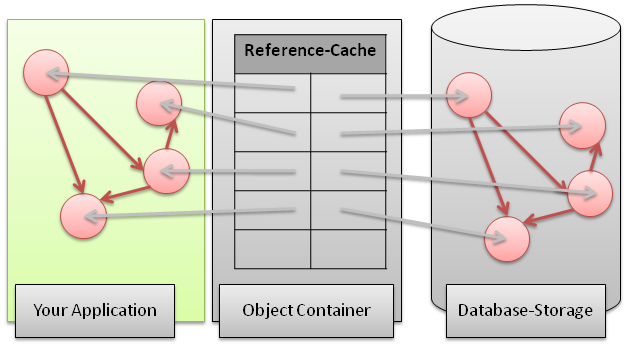
\includegraphics[width=\maxwidth]{images/ref-basics-indentity-concept-reference-cache.png}
\end{center}
\subsubsection*{Weak Reference}

By default db4o uses weak references in the reference cache. While your application has at least one references to an object, the reference cache has reference to it. But as soon as your application has no reference to the object anymore, it can be collected by the garbage collector. db4o will never prevent any object from being garbage collected. In the end persisted objects are garbage collected like any other objects.

To keep the cache clean, db4o does periodically remove all empty weak references. You can configure that clean-up interval. \hyperref[ref:configuration-common-weak-reference-collection-interval]{See "Weak Reference Collection Interval"} (p.~\pageref{ref:configuration-common-weak-reference-collection-interval})

You even can disable the weak reference. \hyperref[ref:configuration-common-disable-weak-references]{See "Disable Weak References"} (p.~\pageref{ref:configuration-common-disable-weak-references}). Then db4o holds regular references to your objects.This prevents the objects from being garbage collected. This means that you need to remove object from the reference cache manually. Or only use short living object containers. \hyperref[ref:advanced-topics-session-containers]{See "Session Containers"} (p.~\pageref{ref:advanced-topics-session-containers})

\subsubsection*{Manually Remove A Object From The Reference Cache}

You can manually remove a object from the reference cache. This only required when you have disabled the \hyperref[ref:configuration-common-disable-weak-references]{weak-references} (p.~\pageref{ref:configuration-common-disable-weak-references}).

\begin{lstlisting}
final Car theCar = container.query(Car.class).get(0);
container.ext().purge(theCar);
\end{lstlisting}

{\small\itshape IdentityConcepts.java: With purge you can remove objects from the reference cache\par}
\medskip

\section{Activation}
\label{ref:basics-activation}

Activation is a db4o mechanism which controls object instantiation. Why is it necessary? Let's look at an example of a stored tree structure. There's one root object, which has a bunch nodes. Each node has again a few subnodes and so on and so forth. What happens when you run a query and retrieve the root object? All the sub-objects will have to be created in the memory! If the tree is very large, this will fill up your memory.

\begin{center}
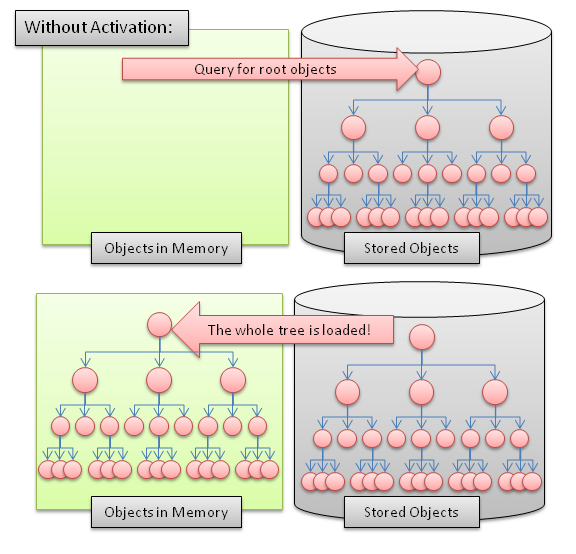
\includegraphics[width=\maxwidth]{images/ref-basics-activation-concept-without-activation.png}
\end{center}
Luckily db4o does not behave like this. When a query returns objects, they are loaded into memory (activated in db4o terms) only to a certain activation depth. In this case depth means "number of member references away from the original object". All the fields beyond the activation depth are set to null or to default values. So db4o does not load the whole object graph. Instead, db4o loads only the parts of the object graph you are interested in.

\begin{center}
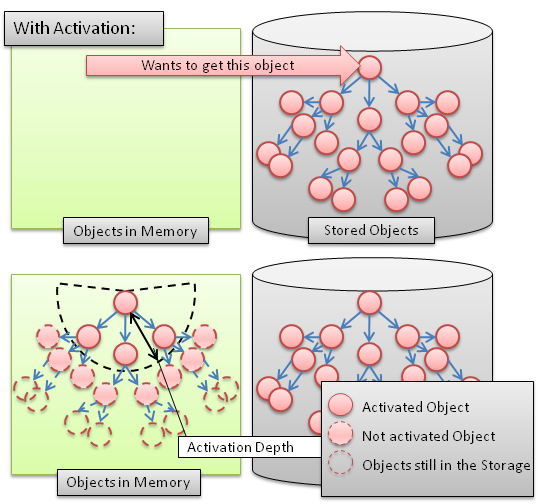
\includegraphics[width=\maxwidth]{images/ref-basics-activation-concept-with-activation.png}
\end{center}
Activation occurs in the following cases:

\begin{enumerate}
\item When you iterate over query results.
\item Object is activated explicitly with the object containers activate method.
\item Collections members are activated automatically, when the collection is activated, using at least depth 1 for lists and depth 2 for maps.
\end{enumerate}

For a concrete example of the activation process: \hyperref[ref:basics-activation-concept-hitting-activation-depth-wall]{See "Activation In Action"} (p.~\pageref{ref:basics-activation-concept-hitting-activation-depth-wall})

If you want to automate the activation process: \hyperref[ref:basics-activation-concept-transparent-activation-framework]{See "Transparent Activation"} (p.~\pageref{ref:basics-activation-concept-transparent-activation-framework})

\subsection{Activation In Action}
\label{ref:basics-activation-concept-hitting-activation-depth-wall}

Let's see db4o's activation in action. To see activation you need a deep object-graph. To keep this example simple we create a person class with a mother-field. This allows us to simply create a very deep object graph.

First the Person class:

\begin{lstlisting}
class Person {
    private Person mother;
    private String name;
    public Person(String name) {
        this.mother = mother;
        this.name = name;
    }

    public Person(Person mother, String name) {
        this.mother = mother;
        this.name = name;
    }

    public Person mother() {
        return mother;
    }

    public String getName() {
        return name;
    }
}
\end{lstlisting}

{\small\itshape Person.java: Person with a reference to the mother\par}
\medskip

After that store a deep hierarchy of persons, for example a hierarchy of seven people. Then query for it and traverse this object graph. When you hit the sixth person, that object won't be activated, because it's outside the activation depth. That object will have all fields set to null.

\begin{lstlisting}
final Person jodie = queryForJodie(container);
Person julia = jodie.mother().mother().mother().mother().mother();
// This will print null
// Because julia is not activated
// and therefore all fields are not set
System.out.println(julia.getName());
// This will throw a NullPointerException.
// Because julia is not activated
// and therefore all fields are not set
String joannaName = julia.mother().getName();
\end{lstlisting}

{\small\itshape ActivationDepthPitfall.java: Run into not activated objects\par}
\medskip

\subsubsection*{Use Explicit Activation}

When you traverse deep object graphs, you might run into not activated objects. Therefore you can activate objects explicitly.

\begin{lstlisting}
Person julia = jodie.mother().mother().mother().mother().mother();
container.activate(julia,5);

System.out.println(julia.getName());
String joannaName = julia.mother().getName();
System.out.println(joannaName);
\end{lstlisting}

{\small\itshape ActivationDepthPitfall.java: Fix with explicit activation\par}
\medskip

\subsubsection*{Configure Activation}

You can configure db4o to increase the activation depth. You can increase it \hyperref[ref:configuration-common-activation-depth]{globally} (p.~\pageref{ref:configuration-common-activation-depth}) or for \hyperref[ref:configuration-objectclass-minimum-activation-depth]{certain classes} (p.~\pageref{ref:configuration-objectclass-minimum-activation-depth}). Or you can \hyperref[ref:configuration-objectclass-cascade-on-activate]{cascade activate} (p.~\pageref{ref:configuration-objectclass-cascade-on-activate}) certain objects.

However remember that activation is there to improve the performance and save memory. If you set the activation depth to high it will hurt the performance.

\subsubsection*{Transparent Activation}

If you have a very complex model or don't want to deal with all the activation hassle then transparent activation is the best option. Transparent activation will manage the activation for you. \hyperref[ref:basics-activation-concept-transparent-activation-framework]{See "Transparent Activation Framework"} (p.~\pageref{ref:basics-activation-concept-transparent-activation-framework})

\subsubsection*{Deactivation}

It's also possible to deactivate an object. When you deactivate an object db4o sets all its fields back to their default value and considers it as deactivated. Deactivation is useful in rare cases where you want to return to the inactivated state for some reason.

\begin{lstlisting}
System.out.println(jodie.getName());
container.deactivate(jodie,5);
// Now all fields will be null or 0
// The same applies for all references objects up to a depth of 5
System.out.println(jodie.getName());
\end{lstlisting}

{\small\itshape ActivationDepthPitfall.java: Deactivate an object\par}
\medskip

\subsection{Transparent Activation}
\label{ref:basics-activation-concept-transparent-activation-framework}

Activation is a db4o-specific mechanism, which controls object instantiation in a query result. Activation works in several modes and is configurable on a database, object or field level. For more information see \hyperref[ref:basics-activation]{Activation} (p.~\pageref{ref:basics-activation}).

Using activation in a project with deep object hierarchies and many cross-references on different levels can make activation strategy complex and difficult to maintain. Transparent activation (TA) project was started to eliminate this problem and make activation automatic in the same time preserving the best performance and the lowest memory consumption.

With transparent activation enabled, objects are fetched on demand and only those that are used are being loaded.

Go to the \hyperref[ref:basics-transparent-persistence]{transparent activation / persistence chapter} (p.~\pageref{ref:basics-transparent-persistence}) to learn more about it.

\section{Update Concept}
\label{ref:basics-update-concept}

Updating objects in db4o is as easy as storing them. You just call then store-method again to update a object. How does a update work? There are two main questions. First, how does db4o recognize a object so that it knows whenever it should update a object or store it as a new object? And what's the scope of updates? All all objects updated? Or just the objects you explicitly store?

\subsection*{Object Recognition}

How does db4o know which object needs to be updated and which object has to be stored as new object? Well db4o uses the \hyperref[ref:basics-identity-concept]{object-identity} (p.~\pageref{ref:basics-identity-concept}) and looks up it if has loaded this object. If the object was loaded by db4o, it is an existing object and will be updated. Otherwise it has to be a new object and is stored as a new object.

\subsection*{Update Depth}

When you update of a object, db4o only stores the changes to a certain depth. This update depth avoids that db4o needs to go through the whole object graph and find out which objects have changed.

By default this update depth is one. This means when you update a object, only the changes on that object are stored. Changes on other objects are not included. When you want to store changes of multiple objects you need either to increase the \hyperref[ref:configuration-common-update-depth]{update-depth} (p.~\pageref{ref:configuration-common-update-depth}), store each object individually or use \hyperref[ref:basics-update-concept-transparent-persistence]{transparent persistence} (p.~\pageref{ref:basics-update-concept-transparent-persistence}).

Take a look at this concrete example to see how the update-depth affects you're operations. \hyperref[ref:basics-update-concept-update-depth-in-action]{See "Update Depth In Action"} (p.~\pageref{ref:basics-update-concept-update-depth-in-action})

Since collection are regular object in db4o the update depth also applies to collections. \hyperref[ref:basics-update-concept-updating-collections]{See "Updating Collections"} (p.~\pageref{ref:basics-update-concept-updating-collections})

If you want to automate the update process of object: \hyperref[ref:basics-update-concept-transparent-persistence]{See "Transparent Persistence"} (p.~\pageref{ref:basics-update-concept-transparent-persistence})

\subsection{Update Depth In Action}
\label{ref:basics-update-concept-update-depth-in-action}

Let's see db4o's update depth in action. We store a few cars with their pilots in the database. Then we update a car and its driver and store the car. The we reopen the database and check if everything was updated. To our surprise the car-name was updated, but the driver isn't. This is the direct result of db4o's update depth policy. It only updates object to a certain update-depth.

\begin{lstlisting}
ObjectContainer container = Db4oEmbedded.openFile(DATABASE_FILE);
try {
    Car car = queryForCar(container);
    car.setCarName("New Mercedes");
    car.getDriver().setName("New Driver Name");

    // With the default-update depth of one, only the changes
    // on the car-object are stored, but not the changes on
    // the person
    container.store(car);
} finally {
    container.close();
}
container = Db4oEmbedded.openFile(DATABASE_FILE);
try {
    Car car = queryForCar(container);
    System.out.println("Car-Name:"+car.getCarName());
    System.out.println("Driver-Name:"+car.getDriver().getName());
} finally {
    container.close();
}
\end{lstlisting}

{\small\itshape UpdateDepthPitfall.java: Update depth limits what is store when updating objects\par}
\medskip

\subsubsection*{Explicitly Store The Driver}

One solution to this issue is to store updated object explicitly, except value objects. So in our case we would store the car and the pilot. This works fine for simple models. However as the model gets more complex this is probably not a feasible solution.

\begin{lstlisting}
Car car = queryForCar(container);
car.setCarName("New Mercedes");
car.getDriver().setName("New Driver Name");

// Explicitly store the driver to ensure that those changes are also in the database
container.store(car);
container.store(car.getDriver());
\end{lstlisting}

{\small\itshape UpdateDepthPitfall.java: Explicitly store changes on the driver\par}
\medskip

There also a variation of this. You can use the store method of the extended container and explicitly state the update depth for the store operation.

\begin{lstlisting}
Car car = queryForCar(container);
car.setCarName("New Mercedes");
car.getDriver().setName("New Driver Name");

// Explicitly state the update depth
container.ext().store(car,2);
\end{lstlisting}

{\small\itshape UpdateDepthPitfall.java: Explicitly use the update depth\par}
\medskip

\subsubsection*{Configure Update Depth}

As alternative you can configure the update depth. You can increase it \hyperref[ref:configuration-common-update-depth]{globally} (p.~\pageref{ref:configuration-common-update-depth}) or for \hyperref[ref:configuration-objectclass-update-depth]{certain classes} (p.~\pageref{ref:configuration-objectclass-update-depth}). It's also possible to enable cascading updates for certain \hyperref[ref:configuration-objectclass-cascade-on-update]{classes} (p.~\pageref{ref:configuration-objectclass-cascade-on-update}) or \hyperref[ref:configuration-objectfield-configuration]{fields} (p.~\pageref{ref:configuration-objectfield-configuration}).

\subsubsection*{Transparent Persistence}

You can get rid of all the update depth troubles by using transparent persistence. In this mode db4o tracks all changes and stores them. \hyperref[ref:basics-update-concept-transparent-persistence]{See "Transparent Persistence"} (p.~\pageref{ref:basics-update-concept-transparent-persistence})

\subsection{Updating Collections}
\label{ref:basics-update-concept-updating-collections}

From the db4o perspective collections behave like ordinary objects. This means that the update-depth also applies to collections. When you change a collection and store the object which contains it, the changes are not stored by default.

\begin{lstlisting}
ObjectContainer container = Db4oEmbedded.openFile(DATABASE_FILE);
try {
    Person jodie = queryForJodie(container);
    jodie.add(new Person("Jamie"));
    // Remember that a collection is also a regular object
    // so with the default-update depth of one, only the changes
    // on the person-object are stored, but not the changes on
    // the friend-list.
    container.store(jodie);
} finally {
    container.close();
}
container = Db4oEmbedded.openFile(DATABASE_FILE);
try {
    Person jodie = queryForJodie(container);
    for (Person person : jodie.getFriends()) {
        // the added friend is gone, because the update-depth is to low
        System.out.println("Friend="+person.getName());
    }
} finally {
    container.close();
}
\end{lstlisting}

{\small\itshape UpdateDepthPitfall.java: Update doesn't work on collection\par}
\medskip

For collections the same rules and \hyperref[ref:basics-update-concept-update-depth-in-action]{settings work as for regular objects} (p.~\pageref{ref:basics-update-concept-update-depth-in-action}). For example when you increase the update depth to two, you can store the parent object and the changes of the collection are persisted as well.

\begin{lstlisting}
EmbeddedConfiguration config = Db4oEmbedded.newConfiguration();
config.common().updateDepth(2);
ObjectContainer container = Db4oEmbedded.openFile(config,DATABASE_FILE);
\end{lstlisting}

{\small\itshape UpdateDepthPitfall.java: A higher update depth fixes the issue\par}
\medskip

\subsection{Transparent Persistence}
\label{ref:basics-update-concept-transparent-persistence}

One of db4o's goals is to make the database transparent to the application logic. Wouldn't it be nice to initially register an object with a single store()-call and then let the database manage all future object modifications? Transparent Persistence does exactly that.It keeps track of changes and stores all modified objects automatically when committing.

This has several benefits:

\begin{itemize}
\item Clean an refactorable code. The code doesn't depend on the right activation-depth.
\item Performance-benefits. Only the objects which are needed are loaded into memory. And only modified objects are stored.
\item No changes can be lost due to miss configured update-depth.
\end{itemize}

To get started go to the \hyperref[ref:basics-transparent-persistence]{transparent activation/persistence topics} (p.~\pageref{ref:basics-transparent-persistence}).

\section{Transparent Activation/Persistence}
\label{ref:basics-transparent-persistence}

One of the challenges of db4o is to manage the \hyperref[ref:basics-activation]{activation of objects} (p.~\pageref{ref:basics-activation}). Also \hyperref[ref:basics-update-concept]{updating} (p.~\pageref{ref:basics-update-concept}) changed objects can be a challenge. The transparent activation/persistence framework solves these issues.

Transparent activation manages the activation of objects. It activates objects as soon as you access them. That means that you don't have to worry about the activation-depth or cascaded activation. As soon as you use transparent activation you don't need to configure any activation depth or cascading updates.

Transparent persistence builds on top of transparent activation and also manages updating objects. It monitors stored objects and memorizes changed objects. When you commit it automatically stores all updated objects. When you use transparent persistence you don't need any update depth nor cascade update configuration.

Transparent activation and persistence are very similar to implement. Therefore the same steps need to be taken to enable them.

To get started take a look at an example. \hyperref[ref:basics-transparentpersistence-ta-enhanced-example]{See "Transparent Persistence Enhanced Example"} (p.~\pageref{ref:basics-transparentpersistence-ta-enhanced-example})

For the learning the implementation details take a look at a manual implementation. \hyperref[ref:basics-transparentpersistence-implementation]{See "Implementation".} (p.~\pageref{ref:basics-transparentpersistence-implementation})

Collections need special attention in transparent activation / persistence. \hyperref[ref:basics-transparentpersistence-collections]{See "Collections".} (p.~\pageref{ref:basics-transparentpersistence-collections})

Also take a look at rollback strategies, which allows db4o to rollback in memory objects. \hyperref[ref:basics-transparentpersistence-automatic-deactivation]{See "Automatic Rollback"} (p.~\pageref{ref:basics-transparentpersistence-automatic-deactivation})

And finally take a look some well known pitfalls: \hyperref[ref:basics-transparentpersistence-transparent-activation-pitfalls]{See "Transparent Activation Pitfalls"} (p.~\pageref{ref:basics-transparentpersistence-transparent-activation-pitfalls})

\subsection{Manual Implementation}
\label{ref:basics-transparentpersistence-implementation}

This topic explains how transparent activation/persistence works and how you can implement the required interfaces manually. In practice you should use the \hyperref[ref:advanced-topics-enhancement-tools]{provided enhancer's} (p.~\pageref{ref:advanced-topics-enhancement-tools}) instead of implementing the interfaces yourself. \hyperref[ref:basics-transparentpersistence-ta-enhanced-example]{See "Transparent Persistence Enhanced Example"} (p.~\pageref{ref:basics-transparentpersistence-ta-enhanced-example})

\subsubsection{Adding the Configuration}
\label{ref:basics-transparentpersistence-implementation:adding}

We need to explicitly configure transparent activation/persistence.

\paragraph*{Transparent Activation}

This adds transparent activation, which automatically activates objects.

\begin{lstlisting}
final EmbeddedConfiguration configuration = Db4oEmbedded.newConfiguration();
configuration.common().add(new TransparentActivationSupport());
ObjectContainer container = Db4oEmbedded.openFile(configuration, DATABASE_FILE_NAME);
\end{lstlisting}

{\small\itshape TransparentPersistence.java: Add transparent activation\par}
\medskip

\paragraph*{Transparent Persistence}

This adds transparent persistence, which automatically activates objects and manages changes on objects. This includes implicitly the transparent activation support.

Optionally you can specify how \hyperref[ref:basics-transparentpersistence-automatic-deactivation]{rollbacks} (p.~\pageref{ref:basics-transparentpersistence-automatic-deactivation}) are handled.

\begin{lstlisting}
final EmbeddedConfiguration configuration = Db4oEmbedded.newConfiguration();
configuration.common().add(new TransparentPersistenceSupport(new DeactivatingRollbackStrategy()));
ObjectContainer container = Db4oEmbedded.openFile(configuration, DATABASE_FILE_NAME);
\end{lstlisting}

{\small\itshape TransparentPersistence.java: Add transparent persistence\par}
\medskip

\subsubsection{Implementing the Activatable Interface}
\label{ref:basics-transparentpersistence-implementation:implemen}

In order to support Transparent Activation, the objects which are stored in the database need to implement the Activatable-interface.

An object which implements the Activatable-interface is responsible for activating itself. For this purpose the class needs a field to keep its activator. This field is only used by the \hyperref[ref:basics-transparent-persistence]{transparent activation/persistence} (p.~\pageref{ref:basics-transparent-persistence}). Therefore it's marked as transient, to avoid that it is stored in the database.

\begin{lstlisting}
import com.db4o.activation.ActivationPurpose;
import com.db4o.activation.Activator;
import com.db4o.ta.Activatable;

public class Person implements Activatable{

    private transient Activator activator;
\end{lstlisting}

{\small\itshape Person.java: Implement the required activatable interface and add activator\par}
\medskip

The implementation of the two methods of the Activatable-interface is straight forward. The bind-method binds an activator to the object. It's called by the transparent activation framework. The activate-method needs to be called before any read or write operation on the object. Since these two methods are always the same, you can move the implementation to a common super class or to a static utility class.

\begin{lstlisting}
public void bind(Activator activator) {
    if (this.activator == activator) {
        return;
    }
    if (activator != null && null != this.activator) {
        throw new IllegalStateException("Object can only be bound to one activator");
    }
    this.activator = activator;
}

public void activate(ActivationPurpose activationPurpose) {
    if(null!=activator){
        activator.activate(activationPurpose);
    }
}
\end{lstlisting}

{\small\itshape Person.java: Implement the activatable interface methods\par}
\medskip

Now to the most important part. Every time a field of the class is accessed you need to call the activate-method with the purpose. This needs to be done in every getter/setter and method. Probably the best way is to use only getter/setter even within the class to access fields. And the getter/setter ensures that the activate-method is called.

\begin{lstlisting}
public void setName(String name) {
    activate(ActivationPurpose.WRITE);
    this.name = name;
}

public String getName()  {
    activate(ActivationPurpose.READ);
    return name;
}

public String toString()  {
    // use the getter/setter withing the class,
    // to ensure the activate-method is called
    return getName();
}
\end{lstlisting}

{\small\itshape Person.java: Call the activate method on every field access\par}
\medskip

Implementing the Activatable-interface manually for every class is repetitive and error prone. That's why this process can be automated.\hyperref[ref:basics-transparentpersistence-ta-enhanced-example]{See "Transparent Persistence Enhanced Example"} (p.~\pageref{ref:basics-transparentpersistence-ta-enhanced-example})

After transparent activation/persistence is enabled you can navigate into object-graph as deeply as you want. The transparent activation will load the objects from the database as you need them. When you've enabled transparent persistence updates are also done transparently.

\begin{lstlisting}
{
    ObjectContainer container = openDatabaseWithTA();
    Person person = Person.personWithHistory();
    container.store(person);
    container.close();
}
{
    ObjectContainer container = openDatabaseWithTA();
    Person person = queryByName(container,"Joanna the 10");
    Person beginOfDynasty = person.getMother();

    // With transparent activation enabled, you can navigate deeply
    // nested object graphs. db4o will ensure that the objects
    // are loaded from the database.
    while(null!=beginOfDynasty.getMother()){
        beginOfDynasty = beginOfDynasty.getMother();
    }
    System.out.println(beginOfDynasty.getName());
    
    container.close();
}
\end{lstlisting}

{\small\itshape TransparentActivationExamples.java: Transparent activation in action\par}
\medskip

\subsubsection{Behavior in Mixed Mode}
\label{ref:basics-transparentpersistence-implementation:behavior}

In some environments there are both, objects which implement the Activatable-interface on other which don't. What's the behavior in this scenario? Then the behavior is this:

\begin{itemize}
\item Objects which implement the Activatable-interface are activated when they are used the first time.
\item Objects which do not implement the Activatable-interface are always fully loaded.
\end{itemize}

That behavior ensures that you never run into not activated objects in the transparent activation / persistence mode.

However objects which do not implement the Activatable-interface are not updated with transparent persistence. You have to do that yourself or enhance those classes as well.

\subsection{Enhancement Example}
\label{ref:basics-transparentpersistence-ta-enhanced-example}

You can inject transparent persistence awareness in your persisted classes without modifying their original code. This is done by enhancing the class-files at build time.

\subsubsection{Required Depedencies}
\label{ref:basics-transparentpersistence-ta-enhanced-example:dependencies}

For transparent activation/persistence you need following dependencies at compile time. (see also the \hyperref[ref:dependency-overview]{dependency overview} (p.~\pageref{ref:dependency-overview}))

\begin{itemize}
\item db4o-8.1-bloat.jar
\item db4o-8.1-instrumentation.jar
\item db4o-8.1-taj.jar
\item db4o-8.1-tools.jar
\end{itemize}

\subsubsection{Enhance Persistent Classes}
\label{ref:basics-transparentpersistence-ta-enhanced-example:enhance}

The first step is to enhance the persisted classes. One possibility is to introduce an Annotation to mark your persisted classes.

By the way, their are alternative way to select the enhanced classes. See  \hyperref[ref:advanced-topics-enhancement-tools-enhancement-for-java-build-time-enhancement]{here} (p.~\pageref{ref:advanced-topics-enhancement-tools-enhancement-for-java-build-time-enhancement}).

\begin{lstlisting}
@Retention(RetentionPolicy.RUNTIME)
@Documented
@Target(ElementType.TYPE)
public @interface TransparentPersisted {
}
\end{lstlisting}

{\small\itshape TransparentPersisted.java: Annotation to mark persisted classes\par}
\medskip

This Annotation is then used to mark all persisted classes.

\begin{lstlisting}
@TransparentPersisted
public class Person {
\end{lstlisting}

{\small\itshape Person.java: Mark your domain model with the annotations\par}
\medskip

The next step is to create a class filter which reports all classes which should be enhanced. There filter checks for the presence of the annotation.

\begin{lstlisting}
public final class AnnotationFilter implements ClassFilter {

    public boolean accept(Class<?> aClass) {
        if(null==aClass || aClass.equals(Object.class)){
            return false;
        }
        return hasAnnotation(aClass)
                || accept(aClass.getSuperclass());
    }

    private boolean hasAnnotation(Class<?> aClass) {
        // We compare by name, to be class-loader independent
        Annotation[] annotations = aClass.getAnnotations();
        for (Annotation annotation : annotations) {
            if(annotation.annotationType().getName()
                    .equals(TransparentPersisted.class.getName())){
                return true;
            }
        }
        return false;
    }

}
\end{lstlisting}

{\small\itshape AnnotationFilter.java: Build a filter\par}
\medskip

\subsubsection*{Enhancing Classes Using Ant}

This enhancement step injects the required bytecode into the domain classes to support transparent activation/persistence.

\begin{lstlisting}
<target name="enhance">
    <!-- Change these according to your project -->
    <property name="target" value="./target/classes/"/>
    <property name="libraries" value="./lib/"/>

    <path id="project.classpath">
        <pathelement path="${target}"/>
        <fileset dir="${libraries}">
            <include name="*.jar"/>
        </fileset>
    </path>

    <!-- We enhance with an additional Ant-run step. You can put this also in an extra file -->
    <typedef resource="instrumentation-def.properties"
             classpathref="project.classpath"
             loaderRef="instrumentation.loader"/>

    <!-- We filter by our annotation -->
    <typedef name="annotation-filter"
             classname="com.db4odoc.tp.enhancement.AnnotationFilter"
             classpathref="project.classpath"
             loaderRef="instrumentation.loader"/>

    <db4o-instrument classTargetDir="${target}"
                  verbose="true">
        <classpath refid="project.classpath"/>
        <sources dir="${target}">
            <include name="**/*.class"/>
        </sources>

        <transparent-activation-step>
            <annotation-filter/>
        </transparent-activation-step>
    </db4o-instrument>
</target>
\end{lstlisting}

{\small\itshape enhance-with-annotation.xml: Ant target for enhancing your classes after building them\par}
\medskip

\subsubsection*{Configure Eclipse to Run Ant Target}

You can configure Eclipse to run the Ant build with each compile step. Right click on your project and choose 'Properties'. Then switch to 'Builders' and add a new one. Choose the 'Ant Builder'. On the new window choose the build-file which contains the example-code. Switch to the 'Targets'-Tab. There choose the enhance-target for the 'Auto-Build'. Now the enhancer-task will be run by Eclipse automatically. The example project above is configured this way.

\subsubsection*{Enhancing Classes Using Maven}

It's also possible to enhance with Maven by using the \href{http://maven.apache.org/plugins/maven-antrun-plugin/}{Ant plugin}.

\begin{lstlisting}
<plugin>
    <artifactId>maven-antrun-plugin</artifactId>
    <version>1.6</version>
    <dependencies>
        <!-- We need the db4o tooling for enhancing stuff -->
        <dependency>
            <groupId>com.db4o</groupId>
            <artifactId>db4o-tools-java5</artifactId>
            <version>8.1-SNAPSHOT</version>
        </dependency>
    </dependencies>
    <executions>
        <execution>
            <phase>compile</phase>
            <configuration>
                <target>
                    <!-- We enhance with an additional Ant-run step. You can put this also in an extra file -->
                    <typedef resource="instrumentation-def.properties"
                             classpathref="maven.compile.classpath"/>

                    <!-- We filter by our annotation -->
                    <typedef name="annotation-filter"
                             classname="com.db4odoc.tp.enhancement.AnnotationFilter"
                             classpathref="maven.compile.classpath"/>

                    <db4o-instrument classTargetDir="target/classes"
                              verbose="true">
                        <classpath refid="maven.compile.classpath"/>
                        <sources dir="target/classes">
                            <include name="**/*.class"/>
                        </sources>

                        <transparent-activation-step>
                            <annotation-filter/>
                        </transparent-activation-step>
                    </db4o-instrument>
                </target>
            </configuration>
            <goals>
                <goal>run</goal>
            </goals>
        </execution>
    </executions>
</plugin>
\end{lstlisting}

{\small\itshape pom.xml: Enhance persisted classes during the build\par}
\medskip

\subsubsection{Check Enhancement}
\label{ref:basics-transparentpersistence-ta-enhanced-example:check}

You can check if the enhancement worked correctly by checking for the activation interface. Such a check should be part of your test-suite to ensure that everything works correctly.

\begin{lstlisting}
if (!Activatable.class.isAssignableFrom(Person.class)) {
    throw new AssertionError("Expect that the " + Person.class + " implements " + Activatable.class);
}
\end{lstlisting}

{\small\itshape TransparentPersistence.java: Check for enhancement\par}
\medskip

\subsubsection{Using Transparent Activation / Persistence}
\label{ref:basics-transparentpersistence-ta-enhanced-example:usingtp}

Configure the transparent activation in order to use it.

\begin{lstlisting}
final EmbeddedConfiguration configuration = Db4oEmbedded.newConfiguration();
configuration.common().add(new TransparentActivationSupport());
ObjectContainer container = Db4oEmbedded.openFile(configuration, DATABASE_FILE_NAME);
\end{lstlisting}

{\small\itshape TransparentPersistence.java: Add transparent activation\par}
\medskip

After that transparent activation is working properly you can transverse along the object graph and don't have to worry about not activated objects:

\begin{lstlisting}
Person person = queryByName(container, "Joanna the 10");
Person beginOfDynasty = person.getMother();

// With transparent activation enabled, you can navigate deeply
// nested object graphs. db4o will ensure that the objects
// are loaded from the database.
while (null != beginOfDynasty.getMother()) {
    beginOfDynasty = beginOfDynasty.getMother();
}
System.out.println(beginOfDynasty.getName());
\end{lstlisting}

{\small\itshape TransparentPersistence.java: Activation just works\par}
\medskip

\subsubsection*{Using Transparent Persistence}

Transparent persistence not only manages the activation, but also manages updating the objects. Configure transparent persistence in order to use it:

\begin{lstlisting}
final EmbeddedConfiguration configuration = Db4oEmbedded.newConfiguration();
configuration.common().add(new TransparentPersistenceSupport(new DeactivatingRollbackStrategy()));
ObjectContainer container = Db4oEmbedded.openFile(configuration, DATABASE_FILE_NAME);
\end{lstlisting}

{\small\itshape TransparentPersistence.java: Add transparent persistence\par}
\medskip

After that updated objects are automatically stored every time you commit.

\begin{lstlisting}
Person person = queryByName(container, "Joanna the 10");
Person mother = person.getMother();
mother.setName("New Name");
// Just commit the transaction. All modified objects are stored
container.commit();
\end{lstlisting}

{\small\itshape TransparentPersistence.java: Just update and commit. Transparent persistence manages all updates\par}
\medskip

\subsection{Collections}
\label{ref:basics-transparentpersistence-collections}

In order to support transparent persistence properly, a class has to implement the Activatable-interface. For your domain classes this is easy to archive. But what about Java-collections? Wouldn't it be nice when collections also work together the transparent activation framework?

db4o brings special, transparent persistence aware collections with it. This collections load the content only when the collections is actually used.

These collections are currently implemented:

\begin{itemize}
\item ActivatableArrayList\textless{}T\textgreater{}: An activatable version of the ArrayList\textless{}T\textgreater{}
\item ActivatableHashMap\textless{}T\textgreater{}: An activatable version of the HashMap\textless{}T\textgreater{}
\item ActivatableHashSet\textless{}T\textgreater{}: An activatable version of the HashSet\textless{}T\textgreater{}
\item ActivatableHashtable\textless{}T\textgreater{}: An activatable version of the HashHashtable\textless{}T\textgreater{}
\item ActivatableLinkedList\textless{}T\textgreater{}: An activatable version of the LinkedList\textless{}T\textgreater{}
\item ActivatableStack\textless{}T\textgreater{}: An activatable version of the Stack\textless{}T\textgreater{}
\item ActivatableTreeSet\textless{}T\textgreater{}: An activatable version of the TreeSet\textless{}T\textgreater{}
\end{itemize}

It's recommended to use the collection-interfaces wherever possible instead of the concrete classes. This avoids unnecessary direct dependencies on the implementations and makes it easy to exchange the implementations.

The enhancement tools can automatically replace the Java-collections with the db4o-equivalent. However there are few rules and limitations. \hyperref[ref:basics-transparentpersistence-collections-enhance-collections]{See "Enhance Collections"} (p.~\pageref{ref:basics-transparentpersistence-collections-enhance-collections})

You can use the db4o-collection directly in your code. For example in the case you implement the transparent activation support manually. Take a looks these tips: \hyperref[ref:basics-transparentpersistence-collections-use-ta-collections]{See "Using Transparent Activatable Collections Directly"} (p.~\pageref{ref:basics-transparentpersistence-collections-use-ta-collections})

\subsubsection{Using TA Collections Directly}
\label{ref:basics-transparentpersistence-collections-use-ta-collections}

You can use the transparent activation aware collections directly in your code. Their behavior is the same as the Java-collections. Here are a few tips:

\begin{itemize}
\item Prefer the collection-interfaces over the concrete classes in your field-, parameter- and return-type declarations. For example declare a field as a List\textless{}T\textgreater{} instead of an ArrayList\textless{}T\textgreater{}
\item Maybe it is useful to create a collection factory in your code. Then you have only one place in your code which decides which implementation is used. That makes it easy to replace the implementations.
\end{itemize}

An example:

\begin{lstlisting}
public class Team  extends AbstractActivatable{ 

    private List<Pilot> pilots = new ActivatableArrayList<Pilot>();

    public boolean add(Pilot pilot) {
        activate(ActivationPurpose.WRITE);
        return pilots.add(pilot);
    }

    public Collection<Pilot> getPilots(){
        activate(ActivationPurpose.READ);
        return pilots;
    }
}
\end{lstlisting}

{\small\itshape Team.java: Using the activation aware collections\par}
\medskip

Currently these collections are available:

\begin{itemize}
\item ActivatableArrayList\textless{}T\textgreater{}: An activatable version of the ArrayList\textless{}T\textgreater{}
\item ActivatableHashMap\textless{}T\textgreater{}: An activatable version of the HashMap\textless{}T\textgreater{}
\item ActivatableHashSet\textless{}T\textgreater{}: An activatable version of the HashSet\textless{}T\textgreater{}
\item ActivatableHashtable\textless{}T\textgreater{}: An activatable version of the HashHashtable\textless{}T\textgreater{}
\item ActivatableLinkedList\textless{}T\textgreater{}: An activatable version of the LinkedList\textless{}T\textgreater{}
\item ActivatableStack\textless{}T\textgreater{}: An activatable version of the Stack\textless{}T\textgreater{}
\item ActivatableTreeSet\textless{}T\textgreater{}: An activatable version of the TreeSet\textless{}T\textgreater{}
\end{itemize}

\subsubsection{Enhance Collections}
\label{ref:basics-transparentpersistence-collections-enhance-collections}

You can use the normal Java-collections in your code and then replace the implementations with the enhancement-tools. \hyperref[ref:basics-transparentpersistence-ta-enhanced-example]{See "Transparent Persistence Enhanced Example"} (p.~\pageref{ref:basics-transparentpersistence-ta-enhanced-example})

The enhancement tools will search for instantiations of collections and replace it with an appropriate transparent activation aware collection.

The transparent persistence aware collections are always subclasses of the Java-collections. Therefore all methods are available. Furthermore potential cast or instanceof checks also work without any problem.

\subsection{Rollback Strategy}
\label{ref:basics-transparentpersistence-automatic-deactivation}

When you \hyperref[ref:basics-acid-and-transactions]{rollback a transaction} (p.~\pageref{ref:basics-acid-and-transactions}) only the state of database affected. The state of the objects in memory isn't touched by the rollback method. Wouldn't it be nice when the objects in memory are also rolled back on a transaction rollback? This can be done by providing a rollback strategy for the transparent persistence. For that you need to pass a RollbackStrategy-implementation to the transparent persistence support. The rollback method will be automatically called once per modified object after a rollback. On the rollback method you can deactivate the modified object. This ensures that the object state is cleared and read again from the database. This is a simple but effective strategy and therefore is implemented in the DeactivatingRollbackStrategy.

\begin{lstlisting}
EmbeddedConfiguration configuration = Db4oEmbedded.newConfiguration();
configuration.common()
        .add(new TransparentPersistenceSupport(new DeactivatingRollbackStrategy()));
\end{lstlisting}

{\small\itshape RollbackExample.java: Configure rollback strategy\par}
\medskip

After adding the rollback strategy objects are rolled back aswell.

\begin{lstlisting}
Pilot pilot = container.query(Pilot.class).get(0);
pilot.setName("NewName");
// Rollback
container.rollback();
// Now the pilot has the old name again
System.out.println(pilot.getName());
\end{lstlisting}

{\small\itshape RollbackExample.java: Rollback with rollback strategy\par}
\medskip

Note that rollback strategies only work for activatable objects.

\subsection{Transparent Activation Pitfalls}
\label{ref:basics-transparentpersistence-transparent-activation-pitfalls}

\hyperref[ref:basics-activation-concept-transparent-activation-framework]{Transparent Persistence} (p.~\pageref{ref:basics-activation-concept-transparent-activation-framework}) is a powerful feature that can make your development much faster, easier and more error-proof. However it can lead to trouble if used in a wrong way. The aim of this chapter is to point you out to typical pitfalls, which lead to unexpected and undesired results.

\subsubsection*{Not Activate Call Before Field Access}

Before accessing any field you need to call the activate-method. This is true for all getter/setter and also for other methods like the toString-method. The best strategy is to call the activate-method in the getter/setter and then access the field through those even in the class itself.

Or use the \hyperref[ref:advanced-topics-enhancement-tools]{enhancement-tools} (p.~\pageref{ref:advanced-topics-enhancement-tools}) to avoid this issue complete.

\subsubsection*{Migrating Between Databases}

\paragraph*{Problem}

Transparent Activation is implemented through the Activatable-interface, which binds an object to the current object container. When an object is stored in more than one object container, this logic won't work, as only one binding is allowed per object.

\paragraph*{Solution}

To allow correct behavior of the object between databases, the object should be unbound before being stored to the another database.Just set the activator to null.

\subsubsection*{Instrumentation Limitations}

\paragraph*{Problem}

For Java built time enhancement the classes to instrument should be on the classpath.

\paragraph*{Solution}

Make sure that all classes to be instrumented are available through the classpath

\subsubsection*{Debugging Instrumented Classes}

Debugging instrumented classes may not work 100\% correct.

You should be able to debug normally anywhere around instrumented bytecode. If you still think that the problem occurs in the instrumented area, please report a bug through the \href{https://github.com/blakemcbride/db4o}{db4o repository}.

\section{Delete Behavior}
\label{ref:basics-delete-behavior}

Deleting an object is as simple as storing an object. You simply call the delete-method on the container to delete it. By default only the object you pass to the delete method is deleted. All referenced objects are not deleted.

\begin{lstlisting}
Car car = findCar(container);
container.delete(car);
// We've deleted the only care there is
assertEquals(0,allCars(container).size());
// The pilots are still there
assertEquals(1,allPilots(container).size());
\end{lstlisting}

{\small\itshape DeletionExamples.java: Deleting object is as simple as storing\par}
\medskip

\subsection*{Reference To Deleted Objects}

What happens when you delete a object which is still referenced by other objects? Well in such cases that reference is set to null.

\begin{lstlisting}
Pilot pilot = findPilot(container);
container.delete(pilot);
\end{lstlisting}

{\small\itshape DeletionExamples.java: Delete the pilot\par}
\medskip

\begin{lstlisting}
// Now the car's reference to the car is set to null
Car car = findCar(container);
assertEquals(null,car.getPilot());
\end{lstlisting}

{\small\itshape DeletionExamples.java: Reference is null after deleting\par}
\medskip

Often you want to ensure that a object isn't referenced anymore, before you can delete it. However such referential integrity isn't supported at the moment. You need to implement your integrity checks manually, for example with \hyperref[ref:advanced-topics-callbacks]{callbacks} (p.~\pageref{ref:advanced-topics-callbacks}).

\subsection*{Cascading Deletion And Collections.}

Additionally you can configure cascading behavior for deletion. \hyperref[ref:basics-delete-behavior-cascading-deletion]{See "Cascading Deletion"} (p.~\pageref{ref:basics-delete-behavior-cascading-deletion})

Also collections are treated like regular objects and need to be deleted explicitly. \hyperref[ref:basics-delete-behavior-collections]{See "Collections And Arrays"} (p.~\pageref{ref:basics-delete-behavior-collections})

\subsection{Cascading Deletion}
\label{ref:basics-delete-behavior-cascading-deletion}

By default db4o only deletes objects which are passed to the delete-method and doesn't delete referenced objects. You can easily change that. Configure the cascading deletion behavior in the configuration for \hyperref[ref:configuration-objectclass-cascade-on-delete]{certain classes} (p.~\pageref{ref:configuration-objectclass-cascade-on-delete}) or \hyperref[ref:configuration-objectfield-configuration]{certain fields} (p.~\pageref{ref:configuration-objectfield-configuration}).

For example we mark that the object in the 'pilot'-field is also deleted:

\begin{lstlisting}
EmbeddedConfiguration config = Db4oEmbedded.newConfiguration();
config.common().objectClass(Car.class).objectField("pilot").cascadeOnDelete(true);
ObjectContainer container = Db4oEmbedded.openFile(config,DATABASE_FILE);
\end{lstlisting}

{\small\itshape DeletionExamples.java: Mark field for cascading deletion\par}
\medskip

When we now delete the car, the pilot of that car is also deleted.

\begin{lstlisting}
Car car = findCar(container);
container.delete(car);
// Now the pilot is also gone
assertEquals(0,allPilots(container).size());
\end{lstlisting}

{\small\itshape DeletionExamples.java: Cascade deletion\par}
\medskip

\subsection{Collections and Arrays}
\label{ref:basics-delete-behavior-collections}

Collections and arrays don't have a special behavior in db4o. When you delete a collection, the collection-members are not deleted. The collection and objects are two independent objects for db4o.

\subsubsection*{Removing From A Collection}

To remove object from a collection you can simple use the regular collection-operations and then store that collection.

\begin{lstlisting}
PilotGroup group = findGroup(container);
final Pilot pilot = group.getPilots().get(0);
group.getPilots().remove(pilot);
container.store(group.getPilots());

assertEquals(3,allPilots(container).size());
assertEquals(2,group.getPilots().size());
\end{lstlisting}

{\small\itshape DeletionExamples.java: Removing from a collection doesn't delete the collection-members\par}
\medskip

\subsubsection*{Remove And Delete Collection Members}

If you want to delete a collection-member, remove it and then delete it.

\begin{lstlisting}
PilotGroup group = findGroup(container);
final Pilot pilot = group.getPilots().get(0);
group.getPilots().remove(pilot);
container.store(group.getPilots());
container.delete(pilot);

assertEquals(2,allPilots(container).size());
assertEquals(2,group.getPilots().size());
\end{lstlisting}

{\small\itshape DeletionExamples.java: Remove and delete\par}
\medskip

\section{Indexing}
\label{ref:basics-indexing}

db4o supports indexes like most databases do. Indexes are data structures which allow efficient lookup of data. When you enable an index, db4o will add an entry to index for each object. This makes the insert and update operation a little slower. However it makes queries a lot faster. A query which uses an index is a order of magnitude faster that a query which cannot use a index.

You can create a index by enabling it on a field. \hyperref[ref:configuration-objectfield-configuration]{See "Adding a Field Index"} (p.~\pageref{ref:configuration-objectfield-configuration})

\begin{lstlisting}
@Indexed
private String zipCode;
\end{lstlisting}

{\small\itshape City.java: Index a field\par}
\medskip

As an alternative you can configure a field index externally.

\begin{lstlisting}
EmbeddedConfiguration configuration = Db4oEmbedded.newConfiguration();
configuration.common().objectClass(Person.class).objectField("name").indexed(true);
\end{lstlisting}

{\small\itshape ObjectFieldConfigurations.java: Index a certain field\par}
\medskip

\subsection*{When And Where Do I Need An Index}

When do you need an index? As a rule of thumb: Add an index all fields which are used in queries. \hyperref[ref:basics-indexing-when-and-where]{See "When And Where"} (p.~\pageref{ref:basics-indexing-when-and-where})

There are different factors which need to be fulfilled to profit from an index.

\begin{itemize}
\item Read operations dominate the database operations: When you application only writes objects but rarely query for objects, there's no benefit of faster queries. However in most system reading is the dominate operation and should be fast.
\item You're using the field / class in a query: If no query touches the field or class you're have a index on, you have not benefit from the index. The index improves only the query performance, but slows down store and update-operations.
\item You actually need a substantial amount of data. The performance gains of an index are negligible for small data sets. When you test indexes use 10'000 and more objects.
\end{itemize}

\subsection{When And Where}
\label{ref:basics-indexing-when-and-where}

When do you need an index? And on which fields do I need an index? An index has a costs and benefits. \hyperref[ref:basics-indexing-costs-and-benefits]{See "Costs And Benefits"} (p.~\pageref{ref:basics-indexing-costs-and-benefits}). Therefore you should only add one when you actually benefit from it.

\subsubsection*{When To Add Queries}

Indexes speed up queries but slow down store and delete operations. You only need to add indexes when queries are too slow. There's no real benefit to add a index when your queries are already fast enough.

Also add index only on fields which are used in queries. Indexes on fields which are never used in a query have no benefit.

\subsubsection*{Where To Add Queries}

How do I find the queries which can benefit from indexes? How do I find queries which couldn't utilize indexes? You can use the \hyperref[ref:configuration-common-diagnostics]{diagnostic-API} (p.~\pageref{ref:configuration-common-diagnostics}) find out. Filter for the LoadedFromClassIndex-message. Every time this message arrives the query didn't use a field index. You can add a break-point to the message-output and find out which query is the source and then add the index.

\begin{lstlisting}
configuration.common().diagnostic().addListener(new DiagnosticListener() {
    @Override
    public void onDiagnostic(Diagnostic diagnostic) {
        if(diagnostic instanceof LoadedFromClassIndex)
        {
            System.out.println("This query couldn't use field indexes "+
                ((LoadedFromClassIndex)diagnostic).reason());
            System.out.println(diagnostic);
        }
    }
});
\end{lstlisting}

{\small\itshape WhereToIndexExample.java: Find queries which cannot use index\par}
\medskip

\subsection{Costs And Benefits}
\label{ref:basics-indexing-costs-and-benefits}

Maintaining an index is additional work and therefore it has its costs. Each time you store a objects which has an index on it, db4o needs to look up the a appropriate place in the index and store a entry there. This costs is paid for each store, update or delete operation. Therefore there's a tradeoff when adding indexes.

The costs are mostly the time consumed to maintain the index. Additionally there's some additional space consumed to store the index. The benefits is that queries which run a order of magnitude faster when using an index.

In practice you should measure and benchmark your solution and check if a index is a benefit to your application. Ensure that you have enough test data. The influence of indexes shows better with a lot of objects. (10'000 and more objects). However since most applications do a lot more read operations than store and update operations adding a index brings a huge benefit.

\subsection{Types And Limitations}
\label{ref:basics-indexing-types-and-limitations}

There are limitations to the db4o indexing. Not all types can be indexed.

\subsubsection*{Types Which Can Be Indexed}

Basically all primitive types like int, long, double etc can be indexed. Indexes on primitive types work extremely well.

Additionally you can index strings, which are handled by db4o like primitives. Strings can be arbitrary long, so a index on string is usually slower than a index on a primitive value. But it's still fast for straight lookups. Note also that a string index can only be used for equality comparison. Comparisons like contains, start with etc don't use the index.

The Date  can also be indexed without any issues.

You also can index any object reference except arrays and strings, which are handled like primitives. This means you can index a field which holds a reference to a object and then look up for objects which have a certain reference.

You can also index BigDecimal and BigNumber objects. Those indexes act like indexes on regular primitive types like int or long. Note that you need to add \hyperref[ref:advanced-topics-type-handling-bigmath]{BigMath-support} (p.~\pageref{ref:advanced-topics-type-handling-bigmath}).

\subsubsection*{Types Which Cannot Be Indexed}

Arrays and collections cannot be indexed. The current db4o index implementation cannot deal with those types. This also means that you cannot do fast look-ups on arrays or collections.

\subsubsection*{Limitations}

Currently the index on strings cannot be used for advanced comparisons like contains, starts with etc.

\subsection{Check For Existing Indexes}
\label{ref:basics-indexing-check-for-index}

Sometime you may want to know if a index exists on a certain field. You can use the \hyperref[ref:advanced-topics-db4o-meta-information]{db4o-meta information} (p.~\pageref{ref:advanced-topics-db4o-meta-information}) to find out if a field is indexed.

\begin{lstlisting}
StoredClass metaInfo = container.ext().storedClass(IndexedClass.class);
// list a fields and check if they have a index
for (StoredField field : metaInfo.getStoredFields()) {
    if(field.hasIndex()){
        System.out.println("The field '"+field.getName()+"' is indexed");
    } else{
        System.out.println("The field '"+field.getName()+"' isn't indexed");
    }
}
\end{lstlisting}

{\small\itshape CheckForAndIndex.java: Check for a index\par}
\medskip

\subsection{Traversing the Index Values}
\label{ref:basics-indexing-traverse-index}

The db4o query processor uses the index to speed up queries. So you just use the query APIs to benefit from indexes. For special cases you might want to traverse the indexed values yourself. You can do this by accessing the index via the \hyperref[ref:advanced-topics-db4o-meta-information]{db4o meta data} (p.~\pageref{ref:advanced-topics-db4o-meta-information}). There you can get the meta-info for a field and then traverse its index. Note that the traverse-method will throw an exception if there is no index available.

\begin{lstlisting}
final StoredField storedField = container.ext()
        .storedClass(Item.class).storedField("data", int.class);
storedField.traverseValues(new Visitor4<Integer>() {
    @Override
    public void visit(Integer fieldValue) {
        System.out.println("Value "+fieldValue);
    }
});
\end{lstlisting}

{\small\itshape TraverseIndexExample.java: Traverse index\par}
\medskip

